% -----------------------------------
% -----------------------------------
% abnTeX2: Normas ABNT NBR 14724:2011 + sugestões FGV/EMAp. 

% Autor: Lauro César Araujo
% Adaptações EMAp: Lucas Machado Moschen 
% Copyright 2012-2018 by abnTeX2 group at http://www.abntex.net.br/ 

%% This work may be distributed and/or modified under the
%% conditions of the LaTeX Project Public License, either version 1.3
%% of this license or (at your option) any later version.
%% The latest version of this license is in
%%   http://www.latex-project.org/lppl.txt
%% and version 1.3 or later is part of all distributions of LaTeX
%% version 2005/12/01 or later.
% ----------------------------------
% ----------------------------------
\documentclass[
	% -- opções da classe memoir --
	12pt,				% tamanho da fonte
	%openright,			% capítulos começam em página ímpar (insere página vazia caso preciso)
	oneside,			% para impressão em recto e verso. Oposto a oneside
	a4paper,			% tamanho do papel. 
	% -- opções da classe abntex2 --
	%chapter=TITLE,		% títulos de capítulos convertidos em letras maiúsculas
	%section=TITLE,		% títulos de seções convertidos em letras maiúsculas
	%subsection=TITLE,	% títulos de subseções convertidos em letras maiúsculas
	%subsubsection=TITLE,% títulos de subsubseções convertidos em letras maiúsculas
	% -- opções do pacote babel --
	english,			% idioma para inglês
	brazil				% idioma para português
	]{abntex2}

%------------------------------------------------
%-------------- Pacotes necessários -------------
%------------------------------------------------

% Escrita 
\usepackage[T1]{fontenc}
\usepackage[utf8]{inputenc}
\usepackage{lmodern}
\usepackage{microtype} % para melhorias de justificação
\usepackage{indentfirst}
\usepackage{multirow}
\usepackage{booktabs}
\usepackage{array}

\renewcommand{\ABNTEXchapterfont}{\fontfamily{ptm}\fontseries{b}\selectfont}

% Gráficos 
\usepackage{color}
\usepackage{caption}
\usepackage{subcaption}
\usepackage{subcaption}
\usepackage{graphicx}

\graphicspath{{../../images/}}

% Matemáticos 
\usepackage{amsthm, amssymb, amsmath, mathtools}
\usepackage{dsfont}

% Outros 
\usepackage{lipsum}
\usepackage{epigraph} 

% Citações 
%\usepackage[brazilian,hyperpageref]{backref}
%\usepackage[alf]{abntex2cite}	% Citações padrão ABNT
\usepackage[style=abnt]{biblatex}
\addbibresource{biblio.bib}  

% \renewcommand{\backrefpagesname}{Citado na(s) página(s):~}
% % Texto padrão antes do número das páginas
% \renewcommand{\backref}{}
% % Define os textos da citação
% \renewcommand*{\backrefalt}[4]{
% 	\ifcase #1 %
% 		Nenhuma citação no texto.%
% 	\or
% 		Citado na página #2.%
% 	\else
% 		Citado #1 vezes nas páginas #2.%
% 	\fi}%
% ---

%----------------------------------------
%------- Capa e Folha de Rosto ----------
%----------------------------------------

\newcommand\subtitulo[1]{\def\@subtitulo{#1}}
\newcommand{\imprimirsubtitulo}{\@subtitulo}

\renewcommand{\imprimircapa}{%
	\begin{capa}%
	\center
		\ABNTEXchapterfont\Large \MakeUppercase{\imprimirinstituicao}
		\\\vspace*{4cm}
		{\ABNTEXchapterfont\large \MakeUppercase{\imprimirautor}}
		\vfill
		\begin{center}
		\ABNTEXchapterfont\large\MakeUppercase{\imprimirtitulo}\normalfont
		%\MakeUppercase{:
		%\imprimirsubtitulo}
		\end{center}
		\vfill
		\normalfont\large\imprimirlocal
		\\\normalfont\large\imprimirdata
		\vspace*{1cm}
	\end{capa}
}

\makeatletter
\renewcommand{\folhaderostocontent}{
  \begin{center}

    %\vspace*{1cm}
    {\ABNTEXchapterfont\large\MakeUppercase{\imprimirautor}}
	
    \vspace*{\fill}\vspace*{\fill}
    \begin{center}
      \ABNTEXchapterfont\bfseries\large\MakeUppercase{\imprimirtitulo}\normalfont%\MakeUppercase{:
      %\imprimirsubtitulo}
    \end{center}
    \vspace*{\fill}
	
    \abntex@ifnotempty{\imprimirpreambulo}{%
      \hspace{7.5cm}
      \begin{minipage}{.5\textwidth}
      	\SingleSpacing
         \imprimirpreambulo
         \\\\
         Orientador: \imprimirorientador
       \end{minipage}%
       \vspace*{\fill}
    }%

    % {\large\imprimirorientadorRotulo~\imprimirorientador\par}
    % \abntex@ifnotempty{\imprimircoorientador}{%
    %    {\large\imprimircoorientadorRotulo~\imprimircoorientador}%
    % }%
    \vspace*{\fill}

    {\large\imprimirlocal}
    \par
    {\large\imprimirdata}
    \vspace*{1cm}

  \end{center}
}
\makeatother

\titulo{Seleção de variáveis por busca estocástica para epidemiologia espacial}
\autor{Isaque Vieira Machado Pim}
\local{Rio de Janeiro}
\data{2022}
\instituicao{%
  Fundação Getulio Vargas \\
  \par
  Escola de Matemática Aplicada
}
\tipotrabalho{Trabalho de Conclusão de Curso}

\preambulo{Trabalho de conclusão de curso apresentada para a Escola de
Matemática Aplicada (FGV/EMAp) como requisito para o grau de bacharel em
Matemática Aplicada. \\ \\ Área de estudo: Estatística Bayesiana Espacial.}

\orientador{Luiz Max Carvalho}

% Se o seu texto tem subtítulo. 
% Se não tiver, altere o arquivo capa_folha_rosto_tex
%\subtitulo{Este é o subtítulo do meu TCC}

%---------------------------------------------
%-------------------- PDF --------------------
%---------------------------------------------

% alterando o aspecto da cor azul
\definecolor{blue}{RGB}{41,5,195}

% informações do PDF
\makeatletter
\hypersetup{
     	%pagebackref=true,
		pdftitle={\@title}, 
		pdfauthor={\@author},
    	pdfsubject={\imprimirpreambulo},
	    pdfcreator={LaTeX with abnTeX2},
		pdfkeywords={abnt}{latex}{abntex}{abntex2}{trabalho acadêmico}, 
		colorlinks=true,       		% false: boxed links; true: colored links
    	linkcolor=blue,          	% color of internal links
    	citecolor=blue,        		% color of links to bibliography
    	filecolor=magenta,      		% color of file links
		urlcolor=blue,
		bookmarksdepth=4
}
\makeatother

% Posiciona figuras e tabelas no topo da página quando adicionadas sozinhas
% em um página em branco. Ver https://github.com/abntex/abntex2/issues/170
\makeatletter
\setlength{\@fptop}{5pt} % Set distance from top of page to first float
\makeatother

%---------------------------------------
%--------- Mais configurações-----------
%---------------------------------------

% Possibilita criação de Quadros e Lista de quadros.
% Ver https://github.com/abntex/abntex2/issues/176
\newcommand{\quadroname}{Quadro}
\newcommand{\listofquadrosname}{Lista de quadros}

\newfloat[chapter]{quadro}{loq}{\quadroname}
\newlistof{listofquadros}{loq}{\listofquadrosname}
\newlistentry{quadro}{loq}{0}

% configurações para atender às regras da ABNT
\setfloatadjustment{quadro}{\centering}
\counterwithout{quadro}{chapter}
\renewcommand{\cftquadroname}{\quadroname\space} 
\renewcommand*{\cftquadroaftersnum}{\hfill--\hfill}

\setfloatlocations{quadro}{hbtp} % Ver https://github.com/abntex/abntex2/issues/176

%-----------------------------------------------------
%--------------------- Margens -----------------------
%-----------------------------------------------------

\setlrmarginsandblock{3cm}{2cm}{*}
\setulmarginsandblock{3cm}{2cm}{*}
\checkandfixthelayout

%-----------------------------------------------------
%------ Espaçamentos entre linhas e parágrafos -------
%-----------------------------------------------------

% O tamanho do parágrafo é dado por:
\setlength{\parindent}{1.3cm}

% Controle do espaçamento entre um parágrafo e outro:
\setlength{\parskip}{0.2cm}  % tente também \onelineskip

% compila o índice
\makeindex

%------------------------------------------------------
%----------- Personal Definitions ---------------------
%------------------------------------------------------

\newcommand{\R}{\mathbb{R}}
\newcommand{\x}{\boldsymbol{x}}
\newcommand{\N}{\operatorname{Normal}}
\newcommand{\betadist}{\operatorname{Beta}}
\newcommand{\bern}{\operatorname{Bernoulli}}
\newcommand{\tril}{\operatorname{tril}}
\newcommand{\eps}{\varepsilon}

\newcommand{\ev}{\mathds{E}}
\newcommand{\var}{\operatorname{Var}}
\newcommand{\cor}{\operatorname{Cor}}
\newcommand{\cov}{\operatorname{Cov}}

\newtheorem{theorem}{Teorema}[]
\newtheorem{proposition}{Proposição}[]
\newtheorem{lemma}{Lema}[]

\theoremstyle{definition}
\newtheorem{definition}{Definição}[section]

\theoremstyle{remark}
\newtheorem*{remark}{Remark}
\newtheorem{assumption}{Assumption}

\newcommand{\improve}[1]{\textcolor{red}{#1}}

%-------------------------------------------------
%----------------- Document ----------------------
%-------------------------------------------------

\begin{document}

\newcounter{num}
% if num != 1, do not print the pre textual 
\setcounter{num}{1}

\selectlanguage{brazil}
\frenchspacing 

%----------------------------------------------
%--------------- Pré-textuais -----------------
%----------------------------------------------
%\pretextual

\imprimircapa

\ifnum\value{num}=1
{\imprimirfolhaderosto*

\begin{fichacatalografica}
	\sffamily
	\vspace*{\fill}					% Posição vertical
	\begin{center}					
	\fbox{\begin{minipage}[c][8cm]{13.5cm}		% Largura
	\small
	Ficha catalográfica elaborada pela BMHS/FGV \\

	%\imprimirautor
	V. M. Pim, Isaque % Paginas com as citações na bibl
	
	\hspace{0.5cm} \imprimirtitulo / \imprimirautor. -- \imprimirdata.
	
	\hspace{0.5cm} \thelastpage f.\\
		
	\hspace{0.5cm}
	\parbox[t]{\textwidth}{\imprimirtipotrabalho~--~Escola de Matemática Aplicada.}\\
	
	\hspace{0.5cm} Advisor: \imprimirorientador .

	\hspace{0.5cm} Includes bibliography. \\
	
	\hspace{0.5cm}
		1. Bioestatística
		2. Estatística Espacial
		2. Seleção de variáveis
		I. Carvalho, Luiz Max
		II. Escola de Matemática Aplicada
		III. \imprimirtitulo 			
	\end{minipage}}
	\end{center}
\end{fichacatalografica}

% Uncomment if you have the pdf 
% \begin{fichacatalografica}
%     \includepdf{fig_ficha_catalografica.pdf}
% \end{fichacatalografica}

%\begin{errata}

\begin{table}[htb]
    \center
    \footnotesize
    \begin{tabular}{|p{1.4cm}|p{1cm}|p{3cm}|p{3cm}|}
    \hline
    \textbf{Folha} & \textbf{Linha} & \textbf{Onde se lê} &
    \textbf{Leia-se}\\
    \hline
    17 & 8 & Matemtica & Matemática \\
    \hline
    \end{tabular}
\end{table}

\end{errata}

\begin{folhadeaprovacao}

    \begin{center}
      {\ABNTEXchapterfont\large\MakeUppercase{\imprimirautor}}
  
      \vspace*{\fill}\vspace*{\fill}
      \begin{center}
        \ABNTEXchapterfont\bfseries\large\MakeUppercase{\imprimirtitulo}\normalfont
        %\MakeUppercase{:
        %\imprimirsubtitulo}	
      \end{center}
      \vspace*{\fill}
      
      \hfill
      \begin{minipage}{.7\textwidth}
          \imprimirpreambulo \\ \\
          E aprovado em 09/12/2022 \\
          Pela comissão organizadora
      \end{minipage}%
      \vspace*{\fill}
     \end{center}
  
     \assinatura{\imprimirorientador \\ Escola de Matemática Aplicada} 
     \assinatura{Dr. Helton Graziadei de Carvalho \\ FGV EMAp}
     \assinatura{Dr. Oswaldo Gonçalves Cruz \\ PROCC/Fiocruz}

     %\assinatura{\textbf{Professor} \\ Convidado 3}
     %\assinatura{\textbf{Professor} \\ Convidado 4}
\end{folhadeaprovacao}

% \begin{folhadeaprovacao}
% \includepdf{folhadeaprovacao_final.pdf}
% \end{folhadeaprovacao}

\begin{dedicatoria}
    \vspace*{\fill}
    %\noindent
    \hfill
    \begin{minipage}{.6\textwidth}
     Dedico essa dissertação aos meus pais: Marcelo e Munira. 
    \end{minipage}
\end{dedicatoria}
 
\begin{agradecimentos}

    Agradeço meus pais, Marcelo e Munira, por razões intermináveis e que não caberiam no escopo desse agradecimento, agradeço por todo amor que nunca me faltou. E meu irmão, Miguel, companheiro e amigo à longa distância. 
    
    Agradeço meus companheiros de turma por toda jornada até aqui. Em especial, meus companheiros do CDMC, que fizeram parte ativa de minha vida no Rio de Janeiro. E meus colegas de tempos passados, que ou ficaram no Espírito Santo, ou também tomaram outros rumos, mas ainda mantém contato
    
    Agradeço o Centro para o Desenvolvimento de Ciências e Matemática (CDMC) da FGV por acreditarem no meu potencial, e custearem todo processo de graduação.
    
    Agradeço meus professores da graduação em Matemática Aplicada da FGV por toda disposição e contribuição com meu crescimento ao longo do curso. 
    
    Destes, agradecimentos especiais ao meu orientador, Luiz Max Carvalho, por não ter faltado em momento algum no desenvolvimento deste trabalho, por todo direcionamento e gama de referências, que certamente me fizeram um acadêmico melhor. E claro, agradeço sua eficiência invejável na comunicação por e-mail.
    
    
    
    
    

\end{agradecimentos}

\begin{epigrafe}
\vspace*{\fill}

\begin{flushright}
    \hspace{7.5cm}
    \textit{
        ``Eu vi uma flor\\
pendida de um galho,\\
banhada de orvalho\\
das noites de abril.\\[5pt]
Se eu fosse um pintor,\\
artista de fato,\\
faria um retrato\\
de flor tão gentil.\\[5pt]
Estava no meio,\\
por entre a folhagem \\
da verde ramagem \\
um tanto escondida.\\[5pt]
Talvez com receio\\
que mãos criminosas,\\
almas venenosas,\\
tirassem- lhe a vida.''} \\
        \textbf{Albércio Vieira Machado}
\end{flushright}
\end{epigrafe}

\setlength{\absparsep}{18pt} 
\begin{resumo}[Resumo]

O mapeamento de doenças tem um longo histórico em vigilância sanitária. Mapas provêm um resumo visual rápido da informação espacial, e permitem encontrar padrões que não apareceriam na forma tabular. Com o aumento da disponibilidade de dados georreferenciados, faz-se necessário o desenvolvimento de técnicas para a análise deste tipo de dados. Do ponto de vista epidemiológico, a modelagem dos padrões e estruturas de correlação, estimação dos parâmetros relevantes para o problema e a comparação de diferentes cenários e a predição para regiões sem observações são essenciais para compreensão do cenário e melhor alocação de recursos para reduzir os impactos de um possível surto.

Neste trabalho, utilizo técnicas modernas, na forma de modelos hierárquicos Bayesianos, para estudar a distribuição do risco para uma doença e análise dos fatores relevantes para a propagação desta doença. O uso de modelos hierárquicos permite de forma robusta e flexível introduzir informações de covariáveis para o modelo, acomodar correlação espacial além de prover uma noção formal da incerteza associada às estimativas de risco. Em especial, consegue conciliar esquemas de seleção de variáveis junto com a estimação dos parâmetros de interesse do modelo.

No \autoref{chap:modelagem} reviso as duas principais técnicas utilizadas ao longo do texto: modelos condicionais autorregressivos (CAR) e seleção bayesiana de variáveis por busca estocástica (BSSVS). Modelos CAR são responsáveis por acomodar estrutura espacial dentro do modelo, enquanto a seleção de variáveis é feita por um esquema de busca estocástica acoplada ao modelo hierárquico. No \autoref{chap:lip}, aplico os métodos desenvolvidos para o caso de câncer labial na Escócia, comparando diferentes modelos e produzindo mapas de risco e quantidades de interesse. No \autoref{chap:ebola}, aplico os métodos desenvolvidos para a epidemia de Ebola na África Ocidental que ocorreu nos anos de 2013-2016. Os dados do Ebola foram enriquecidos com informações filogenéticas como variáveis explanatórias. Os resultados são utilizados para produzir mapas de risco e realizar a predição de áreas sem observações

 Palavras-chave: mapeamento de doenças, modelos hierárquicos bayesianos, seleção de variáveis 
\end{resumo}

\begin{resumo}[Abstract]
 \begin{otherlanguage*}{english}
  Disease mapping has a long history in health surveillance. Maps provide a quick summary of spatial information that otherwise would not pop up in a tabular format. With the increasing quantity of georeferenced data, it is necessary to develop methods and techniques to analyze such data. From an epidemiological point of view, modeling patterns and correlation structures, estimation of the relevant parameters, comparison of different scenarios and prediction of missing data are essential to understand the situation and better allocate resources, reducing damage from a possible disease outbreak.
  

  In this text, I make use of modern methods in the form of Bayesian hierarchical models to study disease burden and analyze the risk factors that are relevant to the spreading of a disease. Hierarchical modeling allows for the introduction of covariate information and adjustment for spatial correlation in a robust and flexible manner. Moreover, it provides a formal notion of uncertainty associated with the risk estimates and allows variable selection schemes along with parameter estimation.

  

  In \autoref{chap:modelagem} I go over the two main methods used in the text: conditional autoregressive (CAR) models and Bayesian Stochastic Search Variable Selection (BSSVS). CAR models are responsible for accommodating spatial information contained in data, and variable selection is done by a stochastic search scheme attached as part of the hierarchical model. In \autoref{chap:lip}, I apply those methods to model the Scottish Lip Cancer case, making comparisons of different modeling options and producing risk maps and quantities of interest. In \autoref{chap:lip}, I apply those methods to model the 2013-2016 West African Ebola epidemic. The data was augmented with phylogenetic information as covariates. The results are then used to produce risk maps and prediction of missing case counts.
 \end{otherlanguage*}

 Keywords: disease mapping, hierarchical modelling, variable selection
\end{resumo}

\pdfbookmark[0]{\listfigurename}{lof}
\listoffigures*
\cleardoublepage

% \pdfbookmark[0]{\listofquadrosname}{loq}
% \listofquadros*
% \cleardoublepage

\pdfbookmark[0]{\listtablename}{lot}
\listoftables*
\cleardoublepage


}\fi

\pdfbookmark[0]{\contentsname}{toc}
\tableofcontents*
\cleardoublepage

% ----------------------------------------------------------
% ELEMENTOS TEXTUAIS
% ----------------------------------------------------------
\textual

\chapter{Introdução}

Nos anos recentes, estudos de mapeamento de doenças se tornaram aplicação rotineira de epidemiologia geográfica, e tipicamente esses estudos são feitos dentro de uma formulação hierárquica Bayesiana \cite{Ribler2019}. Mapas provêm
um resumo visual rápido da informação espacial, e permitem encontrar padrões que não
apareceriam na forma tabular. 
A alocação de recursos para combate a surtos de doenças deve ter como guia básico mapas de zonas de risco para uma doença, e uma lista de possíveis fatores relevantes para a propagação da doença.
Neste texto, reviso e aplico métodos comumente sugeridos para a análise de dados de casos de doença agregados por alguma unidade de área no contexto de mapeamento de doenças e regressão espacial, assim como métodos para seleção de variáveis dentro do esquema de regressão. 

Devemos ter cuidado com regressões espaciais por dois motivos: Primeiro, sempre que tratamos de dados agregados podemos cair na possibilidade de falácia ecológica, e isso só pode ser amenizado com a inclusão de dados a nível de indivíduo. Segundo, quando existe dependência espacial no resíduo, termo que defino no corpo do texto, e quando existe estrutura espacial na variável resposta, então as estimativas de parâmetros vão mudar quando comparadas a um cenário de independência, e os dados por si só não podem acomodar todo tipo de forma e extensão de correlação espacial \cite{Wakefield2007}. Para isso,  o uso de modelos hierárquicos permite de forma robusta e flexível introduzir informações de covariáveis para o modelo, acomodar correlação espacial além de prover uma noção formal da incerteza associada às estimativas de risco. Em especial, consegue conciliar esquemas de seleção de variáveis junto com a estimação dos parâmetros de interesse do modelo.

A divisão do texto é a que segue: no Capítulo 2 reviso as duas principais técnicas utilizadas ao longo do texto: modelos
condicionais autorregressivos (CAR) e seleção bayesiana de variáveis por busca estocástica
(BSSVS). Modelos CAR são responsáveis por acomodar estrutura espacial dentro do
modelo, enquanto a seleção de variáveis é feita por um esquema de busca estocástica
acoplada ao modelo hierárquico. No Capítulo 3, aplico os métodos desenvolvidos para o
caso de câncer labial na Escócia, comparando diferentes modelos e produzindo mapas de
risco e quantidades de interesse. No Capítulo 4, aplico os métodos desenvolvidos para a
epidemia de Ebola na África Ocidental que ocorreu nos anos de 2013-2016. Os dados do
Ebola foram enriquecidos com informações filogenéticas como variáveis explanatórias. Os
resultados são utilizados para produzir mapas de risco e realizar a predição de áreas sem
observações.

% ----------------------------------------------------------
% Finaliza a parte no bookmark do PDF
% para que se inicie o bookmark na raiz
% e adiciona espaço de parte no Sumário
% ----------------------------------------------------------
\phantompart

\chapter{Modelagem}\label{chap:modelagem}

Neste capítulo, detalho os modelos estatísticos empregados neste trabalho, incluindo os módulos espacial e de seleção de variáveis, respectivamente.

\section{Modelos Espaciais}\label{sec:spatial}

\begin{citacao}[english]
{\small ``Geography isn’t just dynamic, it’s a narrative — it shows you a place and tells a story about that place, what’s happening there now, and what will happen next.''\\
\textbf{Jack Dangermond}}
\end{citacao}
% https://www.iso.org/committee/54904.html
A estatística espacial é o ramo da estatística que lida com dados geográficos. Dados geográficos são definidos pela ISO/TC 211 \cite{ISOTC}  como dados contendo de forma implícita ou explícita sua localização relativa à Terra. Para fins de modelagem \cite{Camara2004}, classifico conjuntos de dados espaciais em três tipos básicos:

\begin{itemize}
    \item \textit{Eventos ou Padrões Pontuais} - eventos pontuais aleatórios ocorrendo dentro de um domínio. Exemplos são: localização de crimes, últimos locais onde uma espécie animal rara foi avistada, dados de \textit{IOT (Internet-Of-Things)}.
    \item \textit{Superfícies Contínuas} - também conhecido como dados Geoestatísticos, são referenciados por pontos fixos a partir de amostras coletadas em campo, podendo estar regularmente ou irregularmente distribuídas. Usualmente, este tipo de dado deriva do levantamento de recursos naturais, e que incluem mapas geológicos, topográficos, etc.
    \item \textit{Áreas com Contagens e Taxas Agregadas} - ou dados em área, ou dados em reticulado. Os dados são agregados em unidades de análise, usualmente delimitadas por polígonos que formam uma partição finita de um determinado domínio. Unidades de análise podem ser, por exemplo, estados, municípios, setores censitários. Exemplos de dados em área são população por município, contagem de casos de uma doença por país, votos por setor censitário.
\end{itemize}

Neste trabalho, daremos enfoque para os dados em área. A análise espacial tem como mantra e principal motivador a \textit{Primeira Lei da Geografia} de \cite{Tobler1970}:

\begin{center}
    \textit{``Everything is related to everything else, but near things are more related than distant things''}
\end{center}

Este é o princípio básico de conceitos como a dependência espacial e a autocorrelação espacial.
Tudo está relacionado, porém as coisas mais próximas estão mais relacionadas que as distantes.
Para fazer sentido analítico da Primeira Lei da Geografia, precisamos definir o que queremos dizer com proximidade, e o que queremos dizer com estar relacionado. 

Central para a análise espacial, o conceito de proximidade é poderoso e flexível.
A forma mais comum de representar a noção de proximidade é com relações de distância e conectividade em um plano Euclidiano vazio.
Mas não precisa ser o caso de o espaço ser plano, nem Euclidiano e nem vazio.
O interesse de geógrafos está nos geoespaços \cite{Miller2004}, espaços que podem representar fenômenos na superfície da terra com noções de caminho de menor custo entre pares de objetos bem definidas. \cite{Miller2004} \cite{Miller2003} descrevem diferentes formas de definir proximidade em diferentes espaços. 

Para dados em área, a noção de proximidade comumente usada é a de conectividade, em especial, determinar que duas regiões são vizinhas se compartilham uma fronteira.
Para formalizar esta definição considere um conjunto de regiões $B = \{1, \dots, n\}$.
Denoto a relação de vizinhança por $i \sim j$, uma relação simétrica mas não reflexiva, pois uma área não é vizinha de si mesma.
O conjunto de vizinhos de uma região é denotado por $\delta i$, e o número de vizinhos por $n_{\delta_i}$. A relação de vizinhança também define um grafo em suas regiões (por isso o dado também é referido como reticulado), onde o conjunto de vértices é o próprio $B$, e a aresta $\{i,j\}$ pertence ao grafo se, e só se, $i \sim j$.
A \autoref{fig:ES_mapas} ilustra um mapa e suas relações de vizinhança por meio de um grafo.

\begin{figure}[h]
\centering
\begin{subfigure}{.5\textwidth}
  \centering
  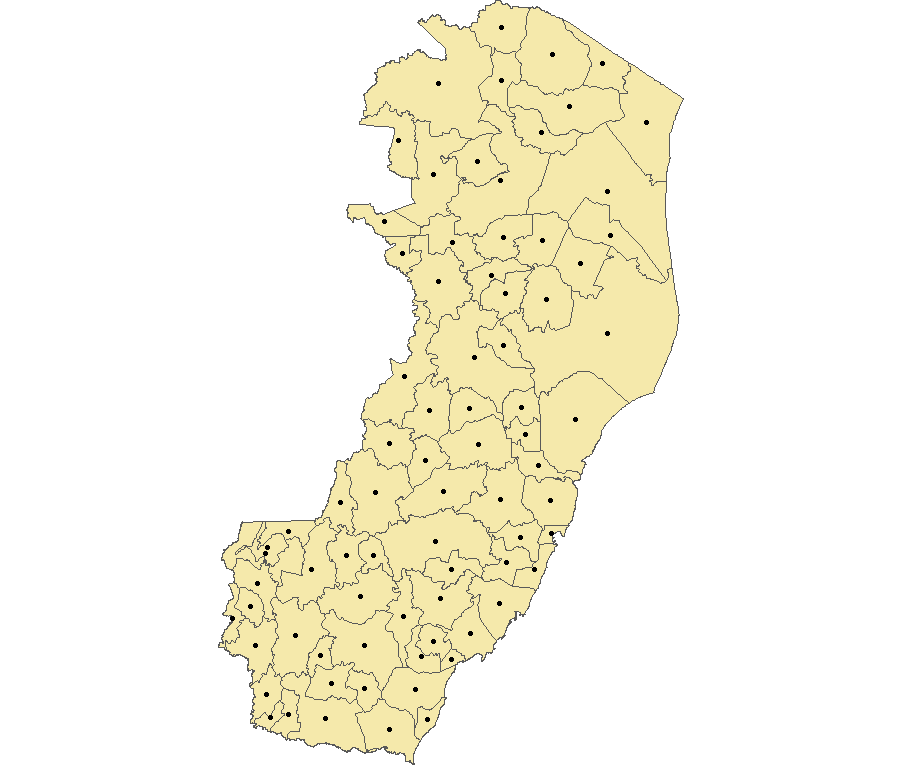
\includegraphics[width=\linewidth]{images/ES_map.png}
  \caption{Mapa apenas com os municípios e seus respectivos centroides.}
  \label{fig:ES}
\end{subfigure}%
\begin{subfigure}{.5\textwidth}
  \centering
  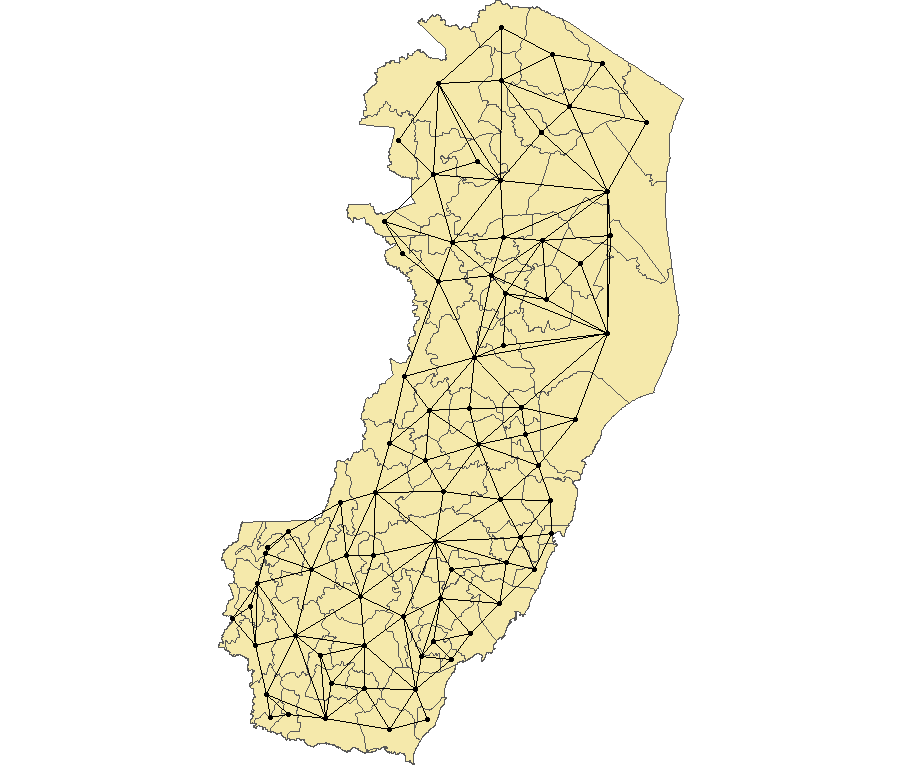
\includegraphics[width=\linewidth]{images/ES_map_conectedgraph.png}
  \caption{Mapa com as relações de vizinhança representadas por um grafo conexo.}
  \label{fig:ES_conexo}
\end{subfigure}
\caption{Mapa dos municípios do Espírito Santo.}
\label{fig:ES_mapas}
\end{figure}

A matriz de adjacências deste grafo é um exemplo de matriz de proximidades.
Uma matriz de proximidades $W$ possui entradas $w_{ij}$ que de alguma forma representam a conexão espacial entre duas regiões $i$ e $j$ (é de costume que $w_{ij} = 0$ se $ i=j$).
Para a matriz de vizinhança, temos $w_{ij} = 1$ se $i\sim j$, e $w_{ij} = 0$ caso contrário.
Há aqui diversas possibilidades para as escolhas de $w_{ij}$, que não necessariamente representam conectividade, como por exemplo $w_{ij}$ ser a distância entre os centroides de $i$ e $j$.
Podemos tomar $w_{ij}  = 1$ se $i$ e $j$ se a distância mínima entre suas fronteias está dentro de um limite pré-estabelecido.
Poderíamos padronizar as linhas de $W$ para torná-la uma matriz estocástica.
O último exemplo acabaria com uma propriedade excelente para uma matriz de proximidades que é ser simétrica. Matrizes de proximidade terão um papel importante para definir a estrutura espacial de nossos modelos.

% Anselin and Griffith (1988) and Arbia  (1989)

E por relacionados para duas entidades geográficas, o que queremos dizer?
No mínimo, esperamos alguma correlação, positiva ou negativa.
Mais do que isso, estarem espacialmente correlacionadas.
Para isso precisamos de técnicas quantitativas para analisar a correlação entre duas variáveis relativa à distância entre as duas ou a conectividade.
Falhar ao levar em conta efeitos espaciais, ou até mesmo ignorá-los pode acarretar em sérios erros na interpretação de modelos como notam \cite{Anselin1988} e \cite{Arbia1989}.
Duas estatísticas padrão para medir a associação espacial entre dados em área são o I de Moran \cite{Moran1950} e o C de Geary \cite{Geary1954}.
São um único valor tentando sumarizar toda associação espacial presente nas áreas.
Para áreas $B = \{1, \dots, n\}$ com observações $Y_i$ para a área $i$, e $w_{ij}$ as entradas da matriz de vizinhança, o I de Moran é dado por

\begin{equation}
    I = \frac{n \sum_{i=1}^n \sum_{j=1}^n w_{ij} (Y_i - \Bar{Y})(Y_j - \Bar{Y})}{(\sum_{i \neq j} w_{ij})\sum_{i=1}^n(Y_i - \Bar{Y})^2},
\end{equation}

e o C de Geary por

\begin{equation}
    C = \frac{(n-1) \sum_{i=1}^n \sum_{j=1}^n w_{ij} (Y_i - Y_j)^2}{2(\sum_{i \neq j} w_{ij})\sum_{i=1}^n(Y_i - \Bar{Y})^2}.
\end{equation}

Estas estatísticas podem ser utilizadas para realizar testes estatísticos.
O I de Moran, sob a hipótese nula que os dados são variáveis i.i.d, é assintoticamente normal com média $-1/(n-1)$.
O C de Geary caso assuma valores baixos entre $(0,1)$ indica a presença de associação espacial.
Assim como o I é assintoticamente normal caso as variáveis sejam i.i.d mas o uso dessas métricas é sugerido apenas como medida exploratória \cite{Li2007}.

Uma forma mais moderna de analisar a dependência espacial de um conjunto de dados é entender que cada unidade de área possui uma quantidade intrínseca de dependência espacial devido à sua situação relativa ao resto do sistema -- ao contrário do I de Moran e do C de Geary, que fornecem uma única medida crua para o sistema inteiro.
A exemplo, temos as estatísticas $G_i$ e $G_i^*$ de \cite{GetisOrd1992}, sobre as quais não entrarei em detalhes.

%Moran's Index	0,145624
%Expected Index	-0,038462
%Variance	0,015644
%z-score	1,471797
%p-value	0,141076

Para exemplificar o uso do I de Moran como ferramenta de detecção de dependência espacial, veja na Figura \ref{fig:pt} o mapa do segundo turno das eleições de 2010 no Brasil.
Calculando o I de Moran para a porcentagem de votos úteis do PT (Partido dos Trabalhadores) e métrica de distância a matriz de vizinhanças, obtemos o valor de $0.1456$ contra o esperado sobre hipótese nula de $-0,0385$, indicando associação espacial entre os estados que elegeram o PT.

\begin{figure}
    \centering
    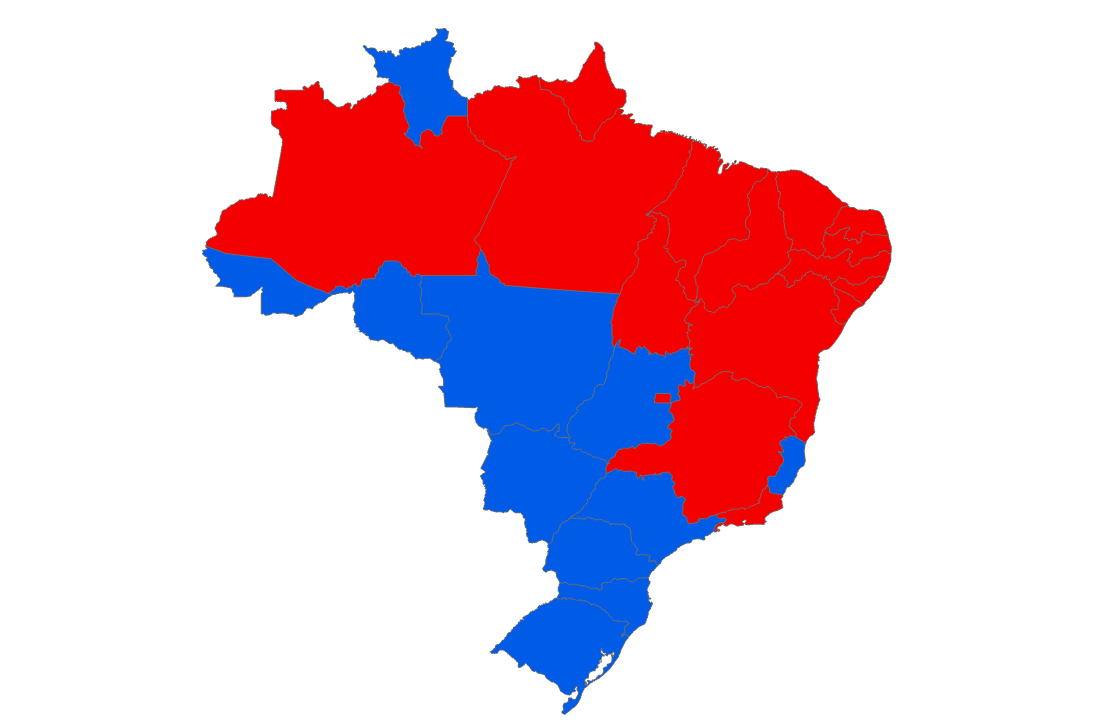
\includegraphics[width = 0.8\linewidth]{images/eleicoes_2010.png}
    \caption{Resultados das eleições de 2010 no Brasil. Em vermelho, estados onde o PT conquistou maioria dos votos. Em azul, maioria do PSDB.}
    \label{fig:pt}
\end{figure}

\cite{Cliff1981} detalha o cálculo de $\mathds{E}[I]$ e $Var(I)$ sob hipótese de normalidade assintótica e de aleatorização.
Aleatorização acontece pois sob hipótese nula não há associação espacial, então permutar as variáveis não modifica a distribuição do $I$ de Moran.
É possível então calcular o \textit{Z-score} e realizar um teste de hipótese.
O teste é implementado em R no pacote \textbf{spdep} como a função \textit{moran.test}.

\subsection{Modelando contagem de casos de uma doença}
% Progressivly explain the Poisson Model?

Para o restante do capítulo, considere a notação $B = \{1, \dots, n\}$ um conjunto de regiões disjuntas, $\delta_i$ o conjunto de vizinhos da região $i$ e $n_{\delta_i}$ o tamanho de $\delta_i$ e $w_{ij}$ como as entradas da matriz de vizinhança $W$.
Dados em área são objetos de forte interesse da Bioestatística e da Epidemiologia.
Tipicamente nos deparamos com dados de contagem de casos por região da seguinte forma:
\[Y_i \quad = \quad \text{casos observados na região $i$,}\quad i=1,\dots,n\]
\[E_i \quad = \quad \text{valor esperado de casos na região $i$,}\quad i=1,\dots,n\]

$Y_i$ variáveis aleatórias e $E_i$ função do número de pessoas em risco na região $i$. 

% Comentar internal standardization

Caso a doença não seja rara \cite{Banerjee2015}, o modelo mais usual é o de Poisson:

\begin{equation}
    \label{eq: poisson}
    Y_i|\theta_i \sim \operatorname{Poisson}(E_i \theta_i),
\end{equation}

onde $\theta_i$ é o risco relativo da região i. Para efeticamente mapear uma superfície de risco, podemos pensar em um modelo de efeito aleatório para os $\theta_i$.
Além de poder assumir que os riscos de cada região vêm de uma mesma distribuição, podemos agregar informação de todas as regiões nas estimativas de risco para uma única região. Também podemos introduzir informação de covariáveis modelando este risco relativo

Considere, então, o seguinte aprimoramento do modelo simples de Poisson, que introduz uma distribuição comum para os $\theta_i$.  

\begin{equation}\label{eq: lognomal}
\begin{split}
    Y_i|\theta_i &\sim \operatorname{Poisson}(E_i \theta_i),\\
    \log(\theta_i) &= \sum_{j=1}^P X_{ij}\beta_j + \varepsilon_i,\\
    \boldsymbol{\varepsilon} &\sim \operatorname{Normal}(0,\Sigma).
\end{split}
\end{equation}

A (log) taxa relativa é modelada como uma componente linear, que introduz informação de covariáveis para o modelo, acrescida de ruído. Aqui $\mathbf{X}$ é uma matriz $N \times P$ com informação de $P$ covariáveis para cada uma das $N$. O ruído modela a sobredispersão, fenômeno muito comum em dados ecológicos e biologia evolucionária \cite{Harrison2014-up}. Esta sobredispersão pode ocorrer devido a covariáveis que não foram incluídas no modelo, excesso de zeros e dados não independentes. Esse rúido é chamado de Efeito Aleatório a Nível Observacional, ou  ORLE (\textit{Observational Level Random Effects}), e ameniza os problemas da sobredispersão descritos. 

% Mix of text from Wakefield and Riebler

Devido à típica incerteza vinda da amostragem, não é recomendado que se analise as taxas diretamente, mas sim tomar ``emprestado'' informação de regiões vizinhas. Espera-se que regiões próximas apresentem mais similaridades que regiões distantes, e é interessante explorar essa informação para extrair estimativas de risco fidedignas.
O efeito é similar a introduzir covariáveis que apresentem tal comportamento: assumem valores similares em locais próximos.
Surge então uma dificuldade para modelar esta dependência espacial, que é conseguir compensar estas covariáveis não observadas e tentar simular seus comportamentos. 

%Riebler
Uma das formas mais comuns de introduzir correlação espacial para um modelo como a Eq. \eqref{eq: lognomal} é com um \textit{Campo de Gaussiano de Markov Intrínseco} (IGMRF), que aqui refiro como modelo CAR (ou termo CAR).
Especificamos a distribuição de um modelo CAR $\boldsymbol{\nu}$ através de suas condicionais completas

\begin{equation*}
    \nu_i | \nu_{-i} \sim \operatorname{Normal}\left(\frac{1}{n_{\delta_i}}\sum_{j \in \delta_i} \nu_j, \frac{1}{n_{\delta_i} \kappa_i}\right),
\end{equation*}

onde $\kappa_i \in (0,+\infty)$ é um parâmetro de precisão.
A partir do Lema de Brook (Lema~\autoref{lema:brook}), e assumindo $\kappa_i = \kappa$ comum parar todas as regiões, podemos derivar a distribuição conjunta de $\nu$:

\begin{equation}
\label{eq: full conditional}
    \pi(\boldsymbol{\nu}|\kappa) \sim \operatorname{Normal}\left(-\frac{1}{2\kappa^2} \sum_{i \sim j} (\nu_i - \nu_j)^2\right) = \operatorname{Normal}\left(\frac{1}{2\kappa^2} \nu^T (D_W - W)\nu \right),
\end{equation}

onde $D_W$ é uma matriz diagonal com entradas $n_{\delta_i}$.
O modelo é intrínseco pois $(D_W - W)1 = 0$, portanto a matriz de precisão é singular e a deficiência de posto é 1 caso o grafo seja conexo, vide \autoref{ap: IGMRF}.
Note também que a densidade é invariante à adição de uma constante, portanto para que não haja confusão com o intercepto, impomos a restrição $\sum_i Y_i = 0$.
Por ser impróprio, vide \autoref{ap: IGMRF}, os modelos CAR intríscos (ICAR) não podem ser usados para modelar dados, e portanto são designadas como prioris.
\cite{Besag1991} mostra que apesar do modelo ser impróprio, a posteriori é própria.

Uma forma de lidar com a condição imprópria do modelo é adicionar um parâmetro $\rho$ escalando a componente $W$  de $(D_W - W)$, controlando então a contribuição espacial deste termo ($W$ é a matriz de vizinhanças). Veja que com $\rho = 0$ temos uma matriz diagonal e, portanto, entradas independentes. Com $\rho = 1$ temos o modelo ICAR. 

\begin{equation}
    \pi(\boldsymbol{\nu}|\kappa) \sim \operatorname{Normal}\left(\frac{1}{2\kappa^2} \nu^T (D_W - \rho W)\nu \right),
\end{equation}

Note que agora tomando $\rho \in (\frac{1}{\lambda_{min}}, \frac{1}{\lambda_{max}})$ obtemos um modelo próprio, onde $\lambda_{min}, \lambda_{max}$ são o menor autovalor e o maior autovalor de $(D_W - \rho W)$, respectivamente
Note que $\rho = 0$ implica em variáveis $\nu_i$ independentes, assim como $\rho = 1$ implica no modelo ICAR.
Apesar de tornar o modelo próprio, permitindo práticas como simulação \textit{a priori} do modelo, o modelo próprio, como alertam \cite{Banerjee2015}, não traz a maleabilidade desejada para introduzir padrões espaciais significativos. 

% Introduzir imagens com simulações de um modelo CAR próprio junto do I e do C


\textcite{Besag1991} introduziram de forma pioneira regressões de Poisson com erros tanto não-estruturados como com erros estruturados de natureza espacial.
O modelo é conhecido como modelo de BYM (Besag-York-Mollié).
Sua formulação é a que segue:

\begin{equation}
    \label{eq: bym}
        Y_i|\theta_i \sim \operatorname{Poisson}(E_i \theta_i),
\end{equation}
\[\log(\theta_i) = \sum_{j=1}^P X_{ij}\beta_j + \xi_i,\]
\[\xi_i = \varepsilon_i + \nu_i,\]
\[\varepsilon_i \sim \operatorname{Normal}(0,\tau_u),\]
\[\nu_i | \nu_{-i} \sim \operatorname{Normal}\left(\frac{1}{n_{\delta_i}}\sum_{j \in \delta_i} \nu_j, \frac{1}{n_{\delta_i} \tau_s}\right).\]

$\tau_s$ e $\tau_u$ parâmetros de precisão.
Note que estes parâmetros de precisão não podem ser vistos de forma independente.
Temos uma observação por área para tentar estimar dois parâmetros! 


\cite{Leroux} e \cite{Dean} trouxeram reparametrizações do modelo BYM para lidar com estes problemas.
Considere a notação $Q = (D_W - W)$ O modelo de Leroux propõe um compromisso entre a componente estruturada e a componente não estruturada por um parâmetro de mistura $\phi \in [0,1]$. O modelo é o BYM mas a componente $\boldsymbol{\xi}$ segue uma distribuição normal com média zero e matriz de covariância

\begin{equation}
\label{eq:leroux}
    \operatorname{Var}(\boldsymbol{\xi}|\tau_b, \phi) = \tau_b^{-1} \left((1-\phi)I + \phi Q  \right)^{-1}.
\end{equation}

A variância condicional do modelo de Leroux é dado pela média ponderada por $\phi$ de $1/\tau_b$ e $1/(\tau_bn_{\delta_i})$.
Como consequência, a decomposição aditiva da variância acontece na log escala do risco relativo condicional à vizinhança da região analisada \cite{Leroux}. O modelo de Dean propõe uma reparametrização do termo $\xi$ do modelo BYM como:
\begin{equation}
\label{eq:dean}
\boldsymbol{\xi} = \frac{1}{\sqrt{\tau_b}}\left( \sqrt{1-\phi}\cdot \boldsymbol{\varepsilon} + \sqrt{\phi} \cdot  \boldsymbol{\nu} \right),
\end{equation}

tendo matriz de covariância
\begin{equation}
    \label{eq:var_dean}
    Var(\boldsymbol{\xi}|\tau_b, \phi) = \tau_b^{-1}\left((1-\phi)I + \phi Q^- \right)
\end{equation}

Onde $Q^-$ denota a inversa generalizada. Esta reparametrização é o modelo BYM com $\tau_s^{-1} = \tau_b^{-1} \phi$ e $\tau_u^{-1} = \tau_b^{-1} (1 - \phi)$. A decomposição aditiva da variância está na log escala do risco relativo.\\

Apesar dos modelos de Leroux e Dean lidarem com a identificação de como a sobredispersão se distribui entre componente estruturada e não estruturada, ambos possuem o problema da componente espacial não estar escalada. Como nota \cite{SORBYE2014}, escalar a componente espacial é essencial para a escolha das prioris, e garantir que as escolhas de priori de uma aplicação possam ser utilizadas em outras aplicações. 

\cite{Ribler2019} detalha o desenvolvimento de um novo modelo BYM, que se atenta à escala. Por simplicidade, considere $\xi$ composto apenas pela componente espacial. Geralmente, as variâncias marginais $\tau_b [Q^-]_{ii}$ dependem da estrutura do grafo analisado. Isso pode ser ilustrado calculando uma variância generalizada, como a média geométrica das variâncias marginais

\begin{equation}\label{eq: GV}
    \sigma^2_{GV} = \exp \left( \frac{1}{n} \sum_{i=1}^n \log \left(  \frac{1}{\tau_b}[Q^-]_{ii}\right) \right).
\end{equation}

Para unificar a interpretação de $\tau_b$ da componente estruturada e da não estruturada, e torná-la transferível entre aplicações, o efeito espacial precisa ser escalado para que $\sigma^2_{GV} = 1/\tau_b$. Isso faz com que o parâmetro $\tau_b$ represente o desvio de um nível constante para qualquer que seja o grafo por trás do modelo. \cite{GMRF} apresenta um esquema para de forma eficiente calcular as entradas da diagonal de $Q^-$. Após extraídos estes componentes, $\sigma^2_{GV}$ é calculado como na \autoref{eq: GV} e é usado para escalar a matriz Q. A partir disso, \cite{Simpson2015}  propõe uma nova parametrização do modelo BYM, que recebe o nome de BYM2. Essa nova parametrização utiliza a componente espacial escalada com precisão 1. O efeito aleatório agora é formulado como

\begin{equation}\label{eq: bym2err}
    \boldsymbol{\xi} = \frac{1}{\sqrt{\tau_b}} \left( \sqrt{1-\phi} \cdot \boldsymbol{\varepsilon} \sqrt{\phi} \cdot \boldsymbol{\nu}^* \right)
\end{equation}

A nova variância é dada por:

\begin{equation}\label{eq: bym2var}
    \operatorname{Var}(\boldsymbol{\xi}|\tau_b, \phi) = \tau_b^{-1}((1-\phi)I + \phi Q_*^-)
\end{equation}

Veja que agora os hiper-parâmetros $\tau_b$ e $\phi$ tem interpretação clara e não são mais confundidos. 

\subsubsection{Escolha das prioris}

Uma questão importante em modelagem bayesiana em geral, e em modelagem espacial em particular é a escolha das distribuições \textit{a priori}.
Modelos GMRF em particular podem ser particularmente sensíveis à especificação de prioris.
%No que se segue, discuto a análise das prioris \textit{via} simulações preditivas.
\textcite{Wakefield2007} trás uma ótima revisão para o caso de regressões espaciais. Par um link log-linear, como é o caso dos modelos estudados nesta seção, é conveniente especificar prioris lognormais para os parâmetros positivos $\exp(\beta_j)$, e fica bem idreto especificar dois quantis e encontrar os parâmetros associados da distribuição lognormal. Denote por $LN(\mu, \sigma)$ a distribuição da lognormal para um parâmetro genérico $\theta$, com $\mathds{E}[\log(\theta)] = \mu$ e $Var(\log(\theta)) = \sigma^2$. Por exemplo, supondo que o risco relativo de uma variável $\beta_j$ tem 50\% de chance de ser menor que 1, podemos assumir \textit{a priori} $\mu = 0$. E uma alta chance, de por exemplo 95\%, de ser menor que 5. Daí $\sigma = \log 5 / 1.645 = 0.98 \approx 1$. Uma priori $e^{\beta_j} \sim LN(0, 1)$ pode ser uma boa escolha. Caso existam muitas covariáveis, ou existe alta correlação entre as covariáveis, vale a pena tornar a priori mais informativa. Como exemplo, veja \cite{IsingDP} que usa prioris de Ising para encorajar a clusterização de variáveis correlacionadas.


Prioris para os parâmetros de precisão do risco relativo residual já não são tão diretas de se derivar. A escolha da distribuição $Gama(a,b)$ para a precisão tanto da componente estruturada, como da não estruturada, ou do risco relativo residual escaldo como no BYM2, é conveniente pois produz uma distribuição marginal em forma fechada. Em especial, sabemos que o modelo de dois níveis
\begin{equation*}
    \xi_i|\tau \sim \operatorname{Normal}(0, 1/\tau), \quad \tau \sim \operatorname{Gama}(a,b)
\end{equation*}

produz distribuição marginal para $\xi_i$ como uma \textit{t}-student generalizada $t_{2a}(0, b/a)$ com $2a$ graus de liberdade, locação zero e escala $b/a$. Uma forma para determinar $a$ e $b$ é especificar um alcance $\exp(\pm R)$ para que o risco residual fique dentro com probabilidade q, e usamos a simetria da t para obter que $\pm t_{q/2}^{2a} \sqrt{b/a} = \pm R$, Onde $\pm t_{q/2}^{2a}$ é o quantil q da t generalizada. Por exemplo, suponha que o risco relativo fique dentro do intervalo (0.5, 2.0) com probabilidade de 95\% , então obtemos que $\tau \sim \operatorname{Gama}(1,0.026)$. 

É importante garantir que a priori acesse todos os possíveis níveis de variabilidade no resíduo. Por esta razão \textcite{Wakefield2007} não recomenda o uso de prioris vagas como $\operatorname{Gama}(0.001,0.001)$.

\subsubsection{Simulações}

Os termos CAR conseguem compensar por covariáveis espacialmente associadas e controlar pela correlação espacial do ruído.
Para ilustrar o fato, considere o seguinte exemplo artificial. Gerei uma covariável $x^*$ com clara dependência espacial para o mapa do Espírito Santo como mostra a \autoref{fig:ES_G}. Em adição foram geradas duas covariáveis $x_1, x_2$ de uma normal padrão para cada região.
A quantidade de interesse $Y$ é então obtida pondo $Y_i \sim \operatorname{Poisson}(\theta_i)$, e $\log(\theta) = 1.5 + 0.5x_1 -0.5x_2 + 0.3x^*$. Vamos amostrar de dois cenários diferentes, desconsiderando a variável $x^*$: o primeiro um modelo Poisson log-normal simples, e o segundo o mesmo modelo com um termo CAR.
Para medir a associação espacial no resíduo utilizo o teste de Moran.
\begin{figure}[ht]
    \centering
    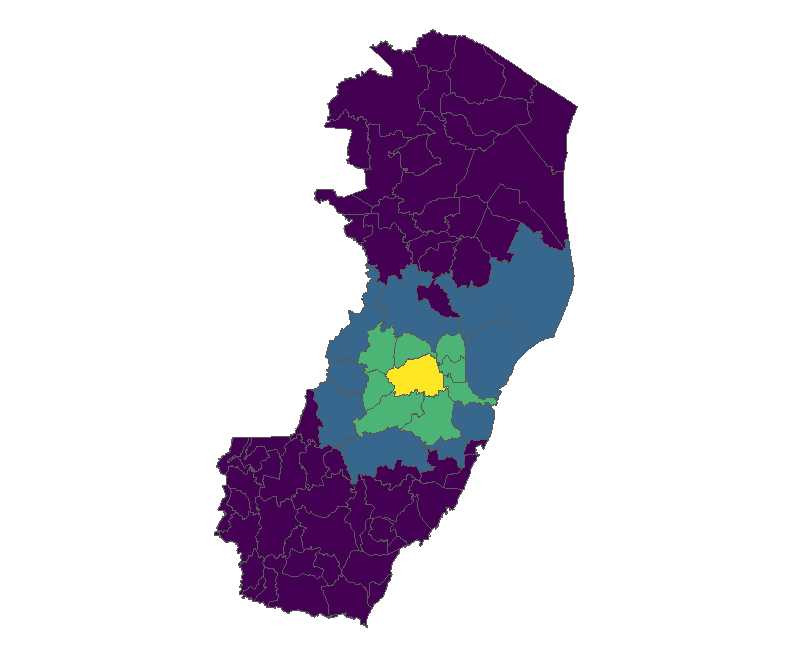
\includegraphics[width = 0.6\linewidth]{images/ES_G.png}
    \caption{Covariável espacialmente correlacionada gerada artificialmente para o mapa do Espírito Santo. }
    \label{fig:ES_G}
\end{figure}
Para o modelo tradicional o I de Moran no resíduo vale 0.194, contra o esperado sobre hipótese nula de -0.013 e um p-valor de 0.0025. Para o modelo com termos CAR o I de Moran no resíduo vale -0.04 contra um esperado de -0.13 e um p-valor de 0.70. 

Um segundo experimento é verificar se as reparametrizações de Dean, Leroux e o BYM2 reduzem aos modelos básicos, i.e, num cenário de alta correlação espacial o parâmetro de mistura $\phi$ se aproximar de 1, no caso de efeitos regionais aleatórios $\phi$ se aproximar de zero. Para isso, simulo do modelo de Poisson com $\log(\theta_i) = 0.4 + 0.5 \xi_i$. Suponho três cenários: $\xi_i$ vindo de uma normal padrão, $\xi$ tendo distribuição $N(0,Q_*^-)$, onde $Q_*$ é a matriz $Q$ escalada para o grafo de adjacências do Espírito Santo, e um terceiro que é uma superfície de risco constante. O modelo avaliado é o BYM2. A priori para o parâmetro $\phi$ é a da indiferença $U(0,1)$.
Os resultados estão apresentados na \autoref{tab:posterior_summary_sim}. Veja que para o modelo de superfície constante o BYM2 a posteriori de $\rho$ não se distancia muito da priori. Já para os cenários de 2 e 3 o parâmetro $\rho$ já apresenta um desvio da priori imposta. Não houve uma redução completa para $\phi = 0$ ou $\phi = 1$. \cite{Simpson2015} propõe o uso de prioris penalizadoras de complexidade (prioris PC) para o BYM2 que conseguem reduzir o parâmetro de mistura para zero. Prioris PC são baseadas na Navalha de Ockham - modelos mais simples devem ser preferidos até que se tenha evidência o suficiente para um modelo mais complexo. 


\begin{table}

\centering
\begin{tabular}{@{}lrrcrrccc@{}}\toprule
& \multicolumn{2}{c}{$\beta_0$} & \phantom{ab}& \multicolumn{2}{c}{$\rho$}&\phantom{ab}& \multicolumn{2}{c}{$\frac{1}{\sqrt{\tau}}$}\\

%\cmidrule{2-3} \cmidrule{5-6}
%& $Média$ & $(upp,lwr)$ && $Média$ & $(upp,lwr)$\\
\midrule
\textbf{Cenário 1} & 0.32 & (0.10) && 0.51 & (0.29) && 0.28 &(0.10)\\
\textbf{Cenário 2} & 0.45 & (0.10) && 0.36 & (0.29) && 0.40 &(0.16)\\ 
\textbf{Cenário 3} & 0.43 & (0.10) && 0.68 & (0.14) && 0.54 &(0.14)\\ 
\bottomrule
\end{tabular}
    \caption{Sumários à posteriori para os 3 cenários descritos: superfície de risco constante, superfície de risco com efeito aleatório regional e superfície de risco com efeito aleatório espacial. Para cada parâmetro temos a mediana à posteriori junto com o desvio-padrão.}
    \label{tab:posterior_summary_sim}
\end{table}





\section{Seleção de Variáveis}

Ao lidar com um conjunto de preditores num termo linear, junto com a estimação dos coeficientes é comum também determinar quais destes preditores estão mais associados com a variável a ser predita. Para o caso de $P$ preditores, queremos determinar um ``bom'' submodelo dentre os $2^P$ submodelos possíveis, baseado em algum critério apropriado .  Para modelos Bayesianos, uma métrica comum para a comparação de modelos é o WAIC (Widely Applicable Information Criterion) \textcite{WAIC}. Usando a mesma notação da \autoref{sec:spatial} para modelos de contagem de casos, considere uma variável de exposição $Y$ para $N$ regiões e um conjunto de $P$ preditores $X = (X_1, \dots, X_p)$ e $\theta$ todos os parâmetros de interesse.
O WAIC  do modelo é calculado como
\begin{equation}
\label{WAIC}
    \operatorname{WAIC} = \mathds{E}[D(\theta)] + 2\sum_{i=1}^N \log(\mathds{E}[p(Y_i|\theta)]) - \mathds{E}[\log p(Y_i|\theta)],
\end{equation}
\[\mathds{E}[D(\theta)] = -2\log(p(Y|\theta))\].

Tem a vantagem de poder ser calculado sem assumir nenhuma distribuição ``verdadeira'', e funciona como um \textit{cross-validation} Bayesiano medindo o poder preditivo do modelo fora da amostra. No entanto, para o trabalho de seleção de variáveis, onde o espaço de modelos cresce exponencialmente com o número de covariáveis, é inviável executar essa computação para todos os modelos.

Do ponto de vista Bayesiano, este problema é contornado ao considerar a seleção de variáveis como uma forma de estimação de parâmetros. A ideia básica é definir as variáveis latentes $\boldsymbol{\gamma} = \{\gamma_i, 1 \leq i \leq P\}$ onde $\gamma_i$ é uma variável indicadora da inclusão do i-ésimo preditor $X_i$ no modelo. Em muitos casos, a decisão de incluir ou não uma variável recai na estimação da probabilidade marginal à posteriori de incluir uma variável no modelo (probabilidade marginal à posteriori dos parâmetros $\gamma_i$). \cite{Ohara2009} traz uma revisão de diversas formas de incluir esta seleção de variáveis para o problema de regressão Bayesiana. Mantendo a notação da \autoref{sec:spatial}, considere agora a seguinte versão aumentada do termo linear da \autoref{eq: lognomal}

\begin{equation}
\begin{split}
        \log(\theta_i) &= \beta_0 + \sum_{j=1}^{P} X_{ij} \nu_j + \varepsilon_i,\\
        \nu_j|\gamma_j, \beta_j &\sim G.
\end{split}
\end{equation}

A tarefa de seleção de variáveis então se simplifica a decidir quais dos parâmetros $\nu_j$ valem zero. A distribuição condicional $G$ seguem, então, a forma de uma mistura ``spike-and-slab'' (pico e platô), possuindo um pico de densidade em zero e um platô de densidade nos outros pontos. Aqui considero dois casos para a densidade $G$. A primeira, de \cite{KM1998} e que me refiro por seleção de variáveis por indicadoras, de forma simples e direta atribui $\nu_j = \gamma_j \beta_j$, e prioris independentes para $\boldsymbol{\gamma}$ e $\boldsymbol{\beta}$. A segunda, inicialmente proposta por \cite{McCulloch1993} e que me refiro como SSVS (Stochastic Search Variable Selection), atribui $\nu_j = \beta_j$ e altera a distribuição de $\beta_j$ baseado nas indicadoras da seguinte forma

\begin{equation}
    \beta_j|\gamma_j \sim (1- \gamma_j) N(0,\sigma^2) + \gamma_j N(0, c_j^2\sigma^2).
\end{equation}


Aqui o pico é uma distribuição centrada em zero com baixa variância, e o parâmetro de $\sigma^2$ é calibrado para que isso aconteça. $c_j$ é calibrado para garantir o platô da distribuição. 

Para todos os casos a escolha da priori para $\gamma$ é parte essencial do problema. Essa escolha deve incorporar qualquer informação prévia sobre os modelos mais plausíveis. No entanto, com $2^P$ modelos isto se torna uma tarefa complexa. Para $\gamma_i$'s independentes com distribuição marginal Bernoulli com $P(\gamma_i = 1) = p_i$ a densidade conjunta de $\gamma$ vale:

\begin{equation}\label{eq:joint_density_gamma}
f(\boldsymbol{\gamma}) = \prod_{i = 1}^{P} p_i^{\gamma_i}(1-p_i)^{1-\gamma_i}.
\end{equation}

Algumas hipóteses de simetria podem facilitar nossa atribuição da priori. A priori uniforme, ou priori da indiferença, é dada por:

\begin{equation}
    f(\boldsymbol{\gamma}) = 2^{-p}.
\end{equation}

Com $p_i = \frac{1}{2}$ para todo $i \in \{1,\dots,P\}$. Podemos também penalizar o tamanho do modelo $M_{\gamma} = \sum_{i=1}^{p} \gamma_i$  pondo mais densidade a priori em modelos menores, favorecendo a parcimônia. Umas das sugestões de \cite{McCulloch1993} é colocar

\begin{equation}
    f(\boldsymbol{\gamma}) = w_{M_{\gamma}} \binom{P}{M_{\gamma}}^{-1},
\end{equation}

onde $w_{M_{\gamma}}$ é a probabilidade a priori de obter um modelo de tamanho $M_{\gamma}$. Para controlar o tamanho do modelo, \cite{Carvalho2019} sugere a parametrização de $p_i$ pela maleabilidade do modelo. Um modelo nada maleável não inclui nenhuma covariável. Seja $w = P(M_{\gamma} = 0)$ nosso parâmetro de maleabilidade. Considerando que $p_i = q, i \in \{1,\dots, P\}$, é fácil ver que $w = (1-q)^P$, e então $q = 1 - w^{1/P}$.

Uma vantagem desta formulação é poder rapidamente avaliar a importância de uma variável por meio do Fator de Bayes de $\gamma$. Podemos escrever o Fator de Bayes para a i-ésima covariável como a razão da razão de chances à posteriori com as chances à priori:

\begin{equation}\label{eq: BF}
BF_i = \frac{\hat{\gamma_i}}{1 - \hat{\gamma_i}}/\frac{p_i}{1-p_i},
\end{equation}

onde $\hat{\gamma_i)}$ é um estimador da probabilidade à posteriori $\gamma_i$.
Para o caso da SSVS, precisamos também definir prioris para $\sigma$. $\sigma$ deve ser tal que $\beta_j \sim N(0,\sigma^2)$ pode ser seguramente substituído por zero. Note que o parâmetro $c_i$ representa a razão das alturas de $N(0,\sigma^2)$ e $N(0,c_i^2\sigma^2)$ em 0. Portanto, pode ser interpretado como a razão de chances de $\beta_i$ ser excluído quando assume valores próximos de 0.  \cite{McCulloch1993} propõe uma alternativa semi-automática, utilizando informação do estimador de mínimos quadrados para $\sigma$. Prefiro não utilizar tal abordagem, adotando prioris mais generalistas para não comprometer a característica Bayesiana completa dos modelos. 

Por fim, precisamos detalhar a escolha de priori para $\beta|\gamma$. Priori para o termo ORLE segue as mesmas recomendações da \autoref{sec:spatial}. Para isso, uso uma normal multivariada

\begin{equation}\label{eq:beta_prior}
    \boldsymbol{\beta}|\boldsymbol{\gamma} \sim N_p(0, D_{\gamma}RD_{\gamma}),
\end{equation}

onde R é a matriz de correlação a priori e 

\begin{equation}\label{eq: Dg}
    D_{\gamma} = \operatorname{diag}[(1-\gamma_1)\tau_1 + \gamma_1 c_1 \tau_1, \dots, (1-\gamma_p)\tau_p + \gamma_p c_p \tau_p].
\end{equation}

Para a escolha de R é interessante observar o efeito dela na matriz de covariância à posteriori de $\beta$, a saber

\begin{equation}\label{eq: posterior_R}
    (\sigma^{-2}X^T X + D_{\gamma}^{-1} R^{-1} D_{\gamma}^{-1})^{-1}.
\end{equation}

Casos notáveis são $R=I$ e $R = (X^T X)^{-1}$. Para o primeiro, os betas ão independentes à priori e as correlações à posteriori serão menores que as correlações da matriz de design. Para o último, correlações à priori e à posteriori serão as mesmas da matriz de design. \cite{McCulloch1993} observa considerável diferença entre ambas as escolhas. Para a escolha $R=I$, modelos menores foram escolhidos com uma maior frequência. 

\subsection{Simulações}

Para avaliar as técnicas de seleção de variáveis vou conduzir algumas simulações artificiais aos moldes de \textcite{VANERP201931}, testando ambos os modelos de Kao e Mallick e o de McCulloch, que me refiro como modelos KM e MC, respectivamente. As simulações são feitas do modelo $y = X^T \boldsymbol{\beta} + \boldsymbol{\varepsilon}, \quad \varepsilon \sim N(0,\sigma^2 I)$ em R com o pacote NIMBLE. Para garantir convergência foi analisado o $\hat{R}$ de Gelman-Rubin, avaliando se o valor para cada parâmetro é menor que 1.05 na última amostra. Todas as cadeias foram executadas com 10.000 iterações, sendo 2.00 usadas como \textit{burn-in}. Como priori para $\sigma^2$ é usado para ambos os modelos uma gama inversa de parâmetros (5,5). Os parâmtros $c$ e $\sigma$ para o modelo MC são fixados como $c = 500$ e $\sigma = 0.01$. Considero que o modelo incluiu uma variável se sua média à posteriori é maior que 0.5


\begin{itemize}
    \item Cenário 1 - $\beta = (3,0,0,-1,0,2,0)$, $\sigma^2 = 9$, X vindo de uma normal multivariada com vetor de média zero, variâncias 1 e correlação entre as variáveis igual a 0.5. São observadas 200 amostras.
    \item Cenário 2 - $\beta = (0.85,0.85,0.85,0.85,0.85,0.85,0.85)$. As outras configurações iguais ao cenário 1.
    \item Cenário 3 - $\beta = (\underbrace{3,\dots,3}_{15},\underbrace{0,\dots,0}_{15})$. $\sigma^2 = 225$. $x_j = Z_1 + w_j,\quad j=1,\dots,5$, $x_j = Z_2 + w_j,\quad j=6,\dots,10$, $x_j = Z_3 + w_j,\quad j=11,\dots,15$, $x_j \sim N(0,1), \quad j=16, \dots 30$. $Z_1, Z_2, Z_3 \sim N(0,1)$ e $w_j \sim N(0,0.01)$. São observadas 200 amostras. 
    \item Cenário 4 - Cenário 3 com 400 amostras.
    \item Cenário 5 - Cenário 3 com $\beta = (\underbrace{3,\dots,3}_{10}, \underbrace{0,\dots,0}_{10}, \underbrace{3,\dots,3}_{10})$ e 40 observações.
\end{itemize}

Para o cenário 1 ambos os modelos geram bons estimadores para os parâmetros da regressão. Já se nota algumas diferenças. O modelo KM ainda tem os betas definidos como zero sendo escolhidos, enquanto o modelo MC rapidamente entende que esses betas não devem ser selecionados. Algo que era esperado, o ESS do modelo MC é menor do que o modelo KM. Para o cenário 2, o modelo KM manteve o mesmo comportamento, aceitando todas as variáveis e fornecendo estimadores razoáveis. Já o modelo MC performou pior, e foi necessário recalibrar os parâmetros $\tau$ e $c$ para obter resultados melhores. Para o cenário 3, o modelo KM incluiu de forma errada 2 variáveis, enquanto do modelo MC incluiu 4 variáveis de forma errada. Para o cenário 4, tivemos4 falsas inclusões para o modelo KM e 6 falsas inclusões para o modelo de MC. Para o cenário 5, 15 falsas inclusões para o modelo de MC e 11 falsas inclusões para o modelo de KM. 

Os resultados das simulações indicam que o modelo de MC precisa de um trabalho mais cuidadoso para a escolha do hiper-parâmetros do problema. Por este motivo, para as simulações praticas utilizo o modelo de KM como método de SSVS. 




\begin{figure}
    \centering
    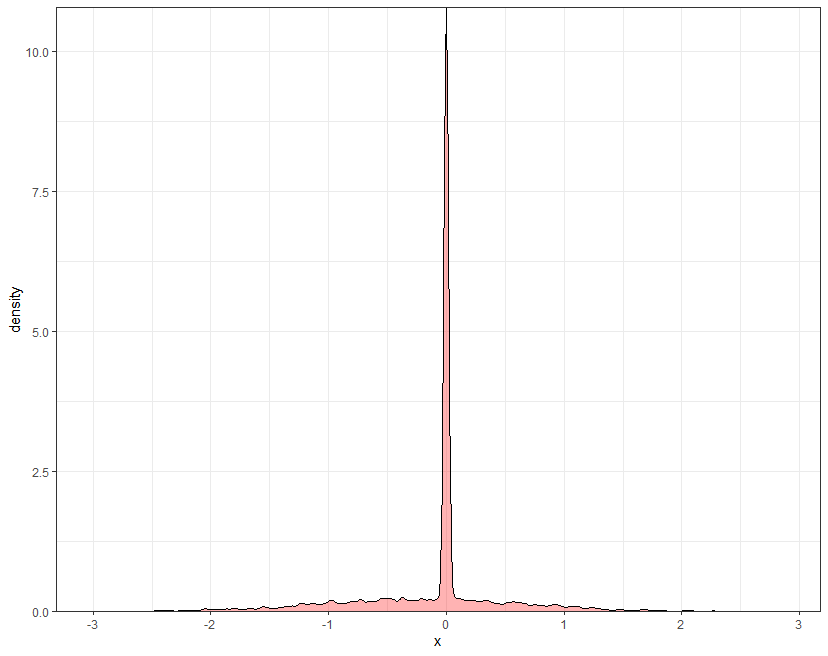
\includegraphics[width = 0.8\linewidth]{images/spike_n_slab2.png}
    \caption{Ilustração da densidade \textit{à posteriori} de uma excluída pra o cenário de simulação 3 para o modelo de Kuo e Mallick. Veja como a concentração de densidade fica em zero, mas o modelo permitiu que ela explorasse outros possíveis valores}
    \label{fig:my_label}
\end{figure}



%\chapter{Seleção e Calibração das Prioris}

\section{Preditiva à priori}
\section{Preditiva à posteriori}
\section{PSA}

\chapter{Aplicação 1: Câncer Labial na Escócia}\label{chap:lip}

\cite{Clayton1987} apresentam dados de casos registrados durante 6 anos (1975-1980) de câncer labial na Escócia.
Para cada um dos 56 condados da Escócia, temos como informação a contagem de casos observados, assim como o "valor esperado" de casos naquela região.
Este valor esperado é obtido através de características demográficas e foram calculados de acordo com \cite{Mantel1968} e aqui são tratados como constantes dadas. 

Ao invés de mapear os casos de câncer, mapeio a SIR (Standard Infection Ratio) em porcentagem para cada condado.
A SIR é dada por:

\begin{equation}
    \label{eq: SIR}
    SIR_i = 100 \times \frac{y_i}{E_i}, \quad i=1,\dots,n
\end{equation}
onde $y_i$ é o número de casos observados e $E_i$ é o valor esperado de casos para o condado $i$. Temos também como covariável a porcentagem a população envolvida em atividades de agricultura, caça e pesca por condado. Ambas as informações estão mapeadas pelas \autoref{fig:SIR Lip cancer} e \autoref{fig:AFF Lip cancer}.
\begin{figure}[b]
\centering
\begin{minipage}{.45\textwidth}
  \centering
  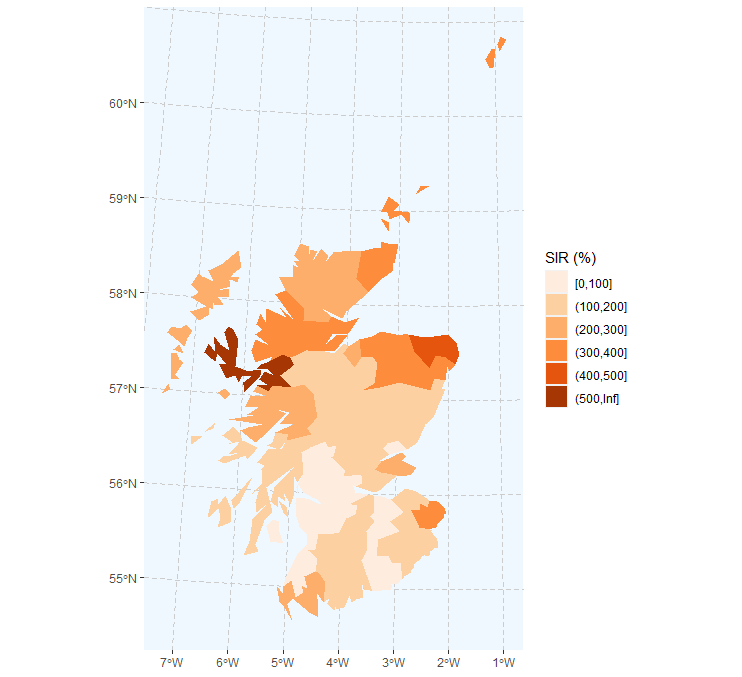
\includegraphics[width=\linewidth]{images/SIR_map_LIP.png}
  \captionof{figure}{Mapa da SIR em porcentagem para os condados da Escócia.}
  \label{fig:SIR Lip cancer}
\end{minipage}%
\begin{minipage}{.45\textwidth}
  \centering
  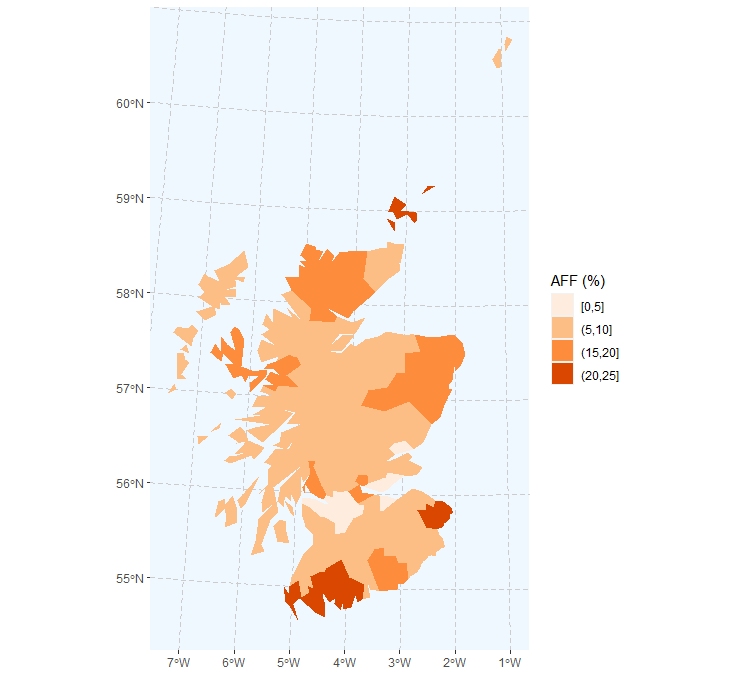
\includegraphics[width=\linewidth]{images/AFF_map_LIP.png}
  \captionof{figure}{Mapa da porcentagem da população envolvida em atividades de agricultura, caça e pesca (AFF).}
  \label{fig:AFF Lip cancer}
\end{minipage}
\end{figure}


Modelo o risco relativo $\theta_i$ em cada condado como

\begin{equation}
    \log(\theta_i) = \beta_0 + \beta_1 \cdot AFF_i + \xi_i,
\end{equation}

onde $\beta_1$ é o efeito da covariável $AFF$ e $\xi_i$ termo de erro para capturar a sobre-dispersão da Poisson. Serão usadas 4 formulações para $\xi_i$ revisadas no Capítulo 2: erro não-estruturado, termo CAR, o modelo de BYM e o modelo BYM2. As simulações da posteriori são feitas utilizando Cadeias de Markov e Monte Carlo. A linguagem utilizada foi R na versão 4.1.3. Para rodar as cadeias, a biblioteca Nimble, versão 0.12.2 e em especial para o calculo do fator de escala do BYM2 o pacote INLA versão 22.05.03. Todas as cadeias foram rodadas para um número fixo de 10.000 iterações com 2.000 iterações de \textit{burn-in}, 4 cadeias em paralelo para cada modelo. Todas as cadeias apresentaram no diagnóstico de Gelman-Rubin  $\hat{R} < 1.05$.\\

Para todos os modelos foram escolhidas prioris vagas  para $\beta_0$ e $\beta_1$, normais de média zero e precisão $10^{-3}$. Todos os modelos também seguem a recomendação de \cite{Sterrantino2018} para modelar casos onde existem ilhas desconectadas (no caso da Escócia, existem 3 ilhas), e modelam a taxa relativa nas ilhas sem componente estruturada.

Os parâmetros de precisão para serem calibrados são $\tau_s$, $\tau_u$ e $\tau_r$, precisão da componente estruturada, precisão da componente não estruturada e precisão conjunta, respectivamente. Seguindo a mesma prática que \cite{Wakefield2007}, atribuo prioris $Gamma(1,0.1)$ para esses parâmetros. Para o parâmetro de mistura $\rho$ do BYM2, a priori não-informativa $Beta(1,1)$. A \autoref{tab:posterior_summary_scotland} mostra o sumário da mediana à posteriori junto com intervalos de credibilidade inferiores e superiores para o intercepto e o coeficiente a covariável AFF. O WAIC de cada modelo também é exibido na tabela. Note que entre os modelos que possuem componente espacial, quase não há diferença entre as estimativas dos parâmetros. A principal diferença entre eles é a interpretabilidade de cada hiperparâmetro, como nota também \cite{Ribler2019}. 

\begin{table}

\centering
\begin{tabular}{@{}lrrcrrcc@{}}\toprule
& \multicolumn{2}{c}{$\beta_0$} & \phantom{ab}& \multicolumn{2}{c}{$\beta_1$}&\phantom{ab}& WAIC\\

%\cmidrule{2-3} \cmidrule{5-6}
%& $Média$ & $(upp,lwr)$ && $Média$ & $(upp,lwr)$\\
\midrule
\textbf{Poisson lognormal} & -0.49 & (-0.80,-0.19) && 6.88 & (3.97, 9.64) && 307.7\\  % var.u 0.59 (0.45 0.78)
\textbf{CAR} & -0.31 & (-0.55, -0.08) && 4.38 & (1.84, 6.82) && 300.2\\ 
% var.s  0.6504600  0.6433667 0.1170732  0.4446273  0.90150079
\textbf{BYM} & -0.33 & (-0.59, -0.07) && 4.94 & (2.22, 7.50) && 303.3\\ 
%var.r  0.4729313  0.4660862 0.0755433  0.3424083  0.64046237
\textbf{BYM2} & -0.32 & (-0.57, -0.06) && 4.60 & (1.74, 7.17) && 298.8\\
\bottomrule
\end{tabular}
    \caption{Sumários à posteriori para os modelos de Câncer Labial na Escócia. Para os parâmetros beta a média a posteriori junto com os intervalos de credibilidade superiores e inferiores de 95\%.}
    \label{tab:posterior_summary_scotland}
\end{table}

Para cada modelo temos também a SIR à posteriori como mostra a \autoref{fig7}. Observe como a componente espacial suaviza o mapa de risco da doença. Além disso, usando o teste de Moran no resíduo destes modelos, obtive O I de Moran com valor 0.21, contra um esperado de -0.019 (p-valor 0.006), alto indício de dependência espacial no resíduo. Já no modelo de BYM a estatística de Moran cai para -0.004 (p-valor de 0.86), ou seja, evidenciando uma diminuição da dependência espacial do resíduo, o que melhora a interpretação dos parâmetros do modelo \cite{Wakefield2007}.

Vale notar o parâmetro $\rho$ do modelo BYM2, que controla a mistura entre erro estruturado e não estruturado. A priori supuz indiferença para este parâmetro, e comecei as cadeias com valores de $\rho$ diferentes, variando a contribuição de cada tipo de erro. A posteriori converge para uma concentração maior de erro estruturado. A mediana à posteriori de $\rho$ foi $0.83 (0.36,0.99)$, o que pode explicar o Modelo de Besag ter tido um WAIC menor (afinal, ele possui erro estruturado puro). A vantagem do BYM2 é poder agora analisar o parâmetro $\tau_r$ e entender quanto da SIR à posteriori foi explicada pelo erro. Lembrando que o erro tem média constante zero, a mediana do desvio padrão à posteriori vale $0.47 (0.34, 0.64)$. 
\begin{figure}[ht] 
  \begin{subfigure}[b]{0.5\linewidth}
    \centering
    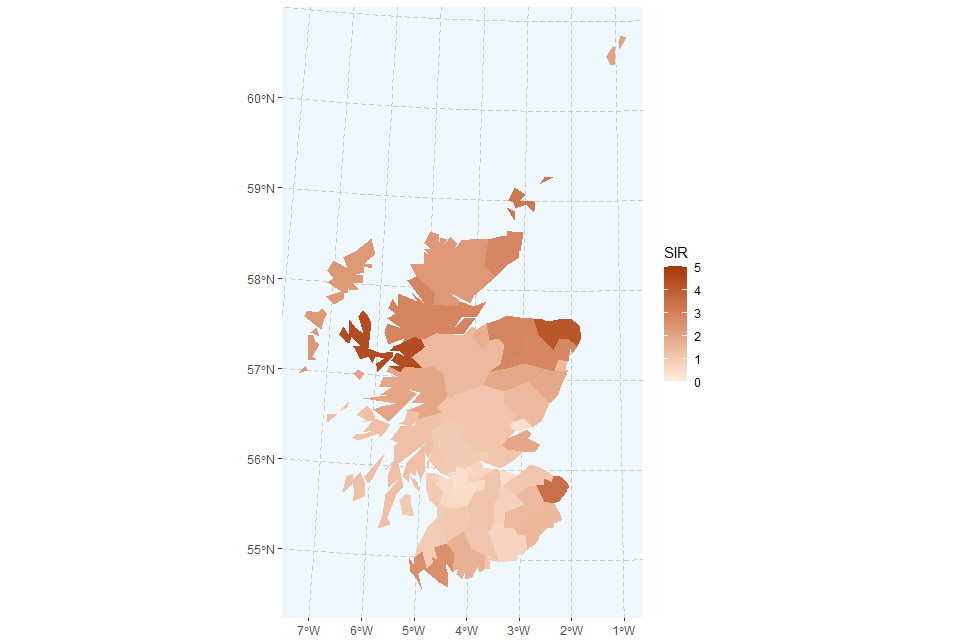
\includegraphics[width=0.9\linewidth]{images/SIR_posteriori_noCAR.png} 
    \caption{Modelo Poisson log-normal puro} 
    \label{fig7:a} 
    \vspace{4ex}
  \end{subfigure}%% 
  \begin{subfigure}[b]{0.5\linewidth}
    \centering
    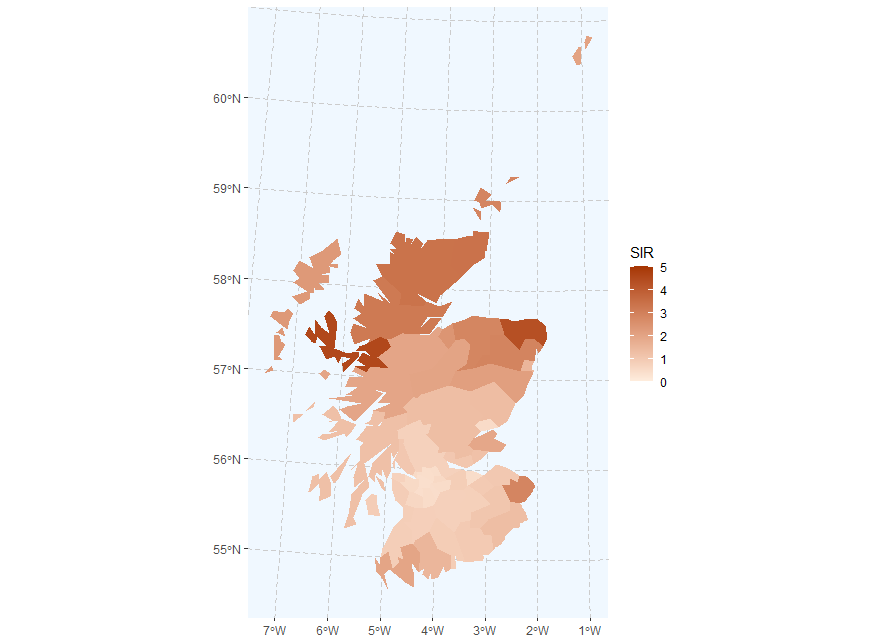
\includegraphics[width=0.9\linewidth]{images/SIR_posteriori_CAR.png} 
    \caption{Modelo de Besag} 
    \label{fig7:b} 
    \vspace{4ex}
  \end{subfigure} 
  \begin{subfigure}[b]{0.5\linewidth}
    \centering
    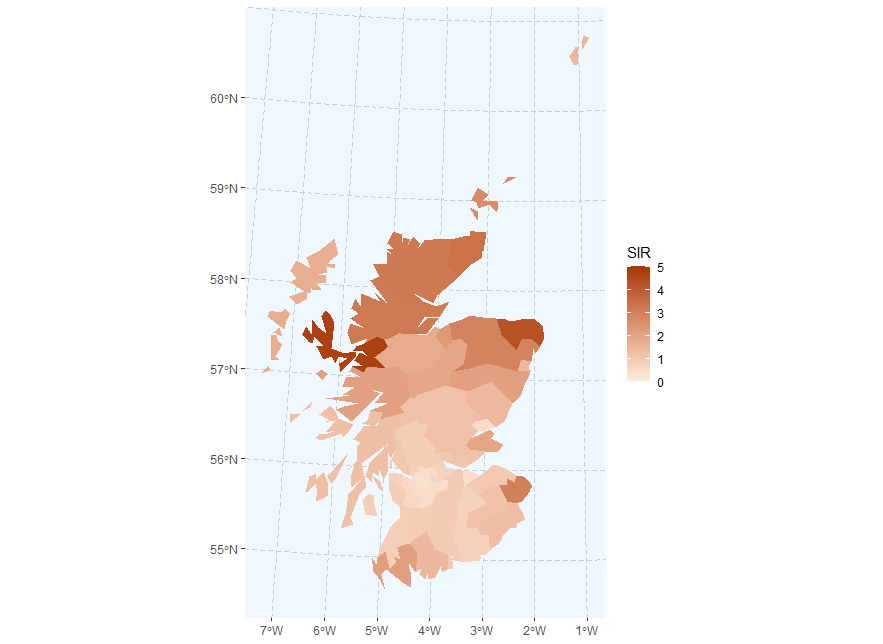
\includegraphics[width=0.9\linewidth]{images/SIR_posteriori_BYM.png} 
    \caption{Modelo BYM} 
    \label{fig7:c} 
  \end{subfigure}%%
  \begin{subfigure}[b]{0.5\linewidth}
    \centering
    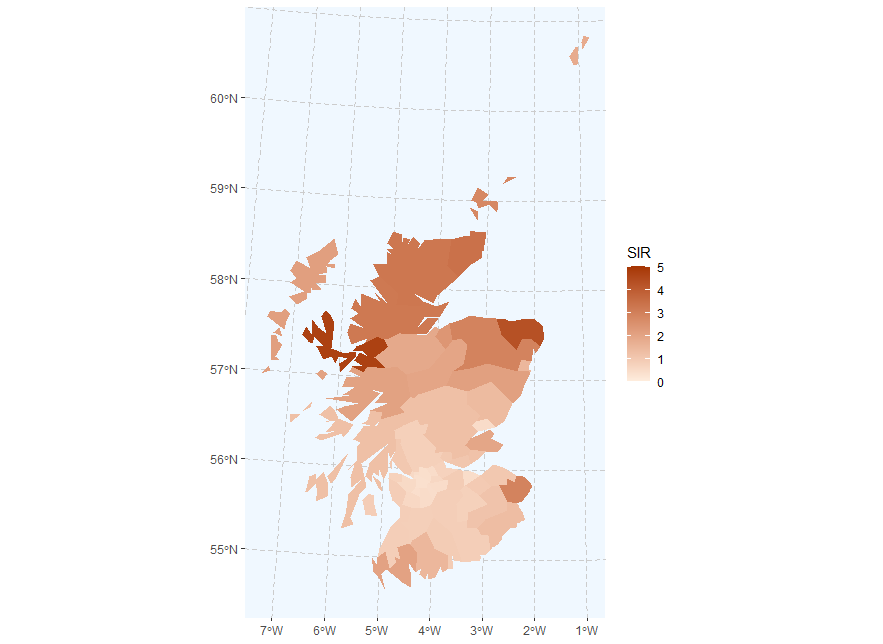
\includegraphics[width=0.9\linewidth]{images/SIR_posteriori_BYM2.png} 
    \caption{Modelo BYM2} 
    \label{fig7:d} 
  \end{subfigure} 
  \caption{SIR à posteriori média para cada um dos modelos analisados. Observe como o modelo sem componente espacial possui o mapa da SIR bem similar ao da taxa crua, e como os modelos espaciais distribuem o efeito da doença para as vizinhanças, promovendo suavização.}
  \label{fig7} 
\end{figure}


Uma última análise interessante é verificar a probabilidade à posteriori da SIR em um determinado condado ser maior que 1. A figura trás essa visualizacão para o modelo BYM2.

\begin{figure}[h]
    \centering
    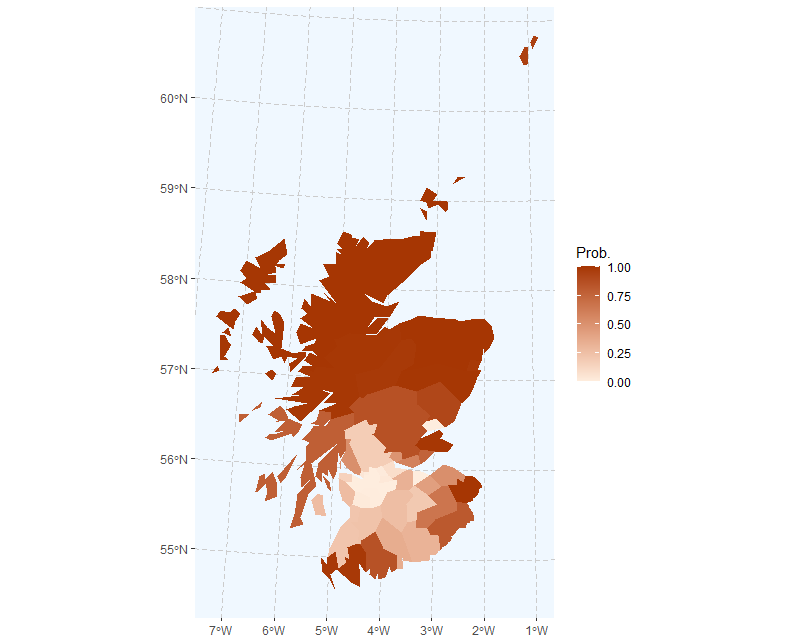
\includegraphics[width = 0.8\linewidth]{images/prob_greater_1.png}
    \caption{Probabilidade à posteriori da SIR ser maior que 1 (modelo BYM2)}
    \label{fig:my_label}
\end{figure}

\chapter{Aplicação 2: Epidemia de Ebola na África Ocidental}\label{chap:ebola}


Em meados de março de 2014 os primeiros casos de Ebola foram detectados na Guiné, e futuras investigações epidemiológicas iriam sugerir que os primeiros casos ocorreram por volta de Dezembro de 2013. Em março de 2016, já se somavam 28.816 suspeitas, possibilidades e casos confirmados de Ebola em Guiné, Libéria e Serra Leoa, com 11.310 mortes. Isso marca a epidemia de Ebola do período de 2013-2016 como uma das piores na história \cite{Carvalho2019}. Isso pois o Ebola já tem casos registrados desde 1976, o primeiro deles na República Democrática do Congo. A pergunta científica que se faz então é: quais foram os fatores relevantes para o considerável aumento repentino do número de casos e de sua propagação geográfica. Para isso, vamos utilizar as técnicas desenvolvidas ao longo do texto para lidar com este problema. 

Seguindo os estudos de \cite{Carvalho2019}, um rico conjunto de dados socioeconômicos, climáticos e genéticos foi disponibilizado. Os dados vem agregados em área para os distritos da Serra Leoa, prefeituras da Guiné e condados da Libéria. Das 81 localidades resultantes, 63 reportaram 1 ou mais casos de Ebola. Essas regiões estão dispostas na \autoref{fig: mapa_ebola}.

\begin{figure}[h]
    \centering
    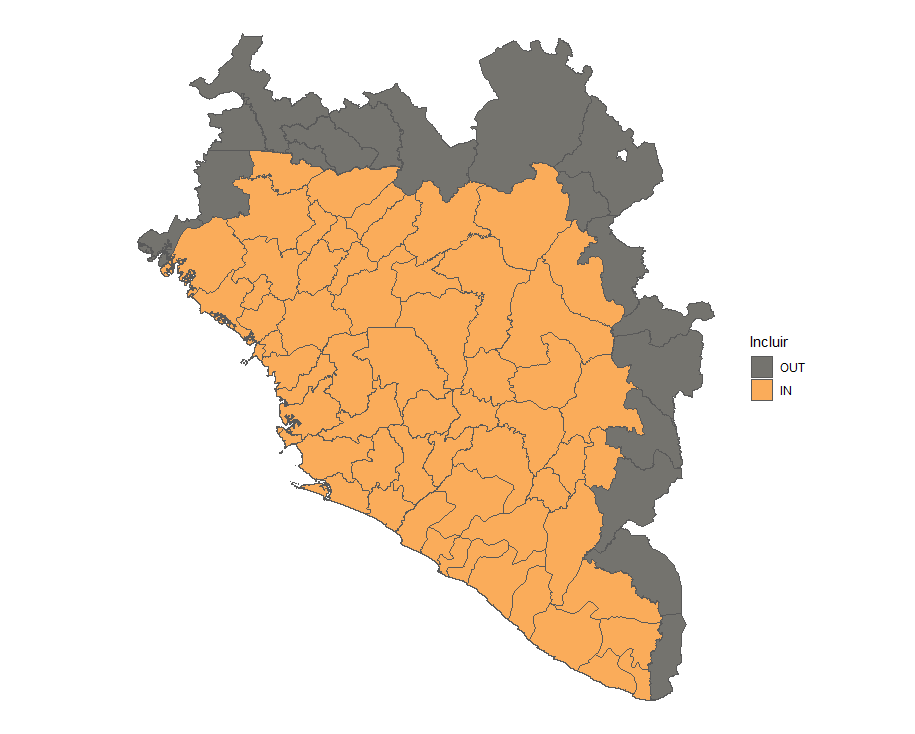
\includegraphics[width = 0.8\linewidth]{images/ebola_regions.png}
    \caption{Regiões da África Ocidental consideradas no modelo. Regiões com a marcação IN registraram 1 ou mais casos de Ebola. }
    \label{fig: mapa_ebola}
\end{figure}

 Os preditores utilizados estão disponíveis na \autoref{tab:ebola_predictors}. 

\begin{figure}
    \centering
    \begin{minipage}{0.45\textwidth}
        \centering
        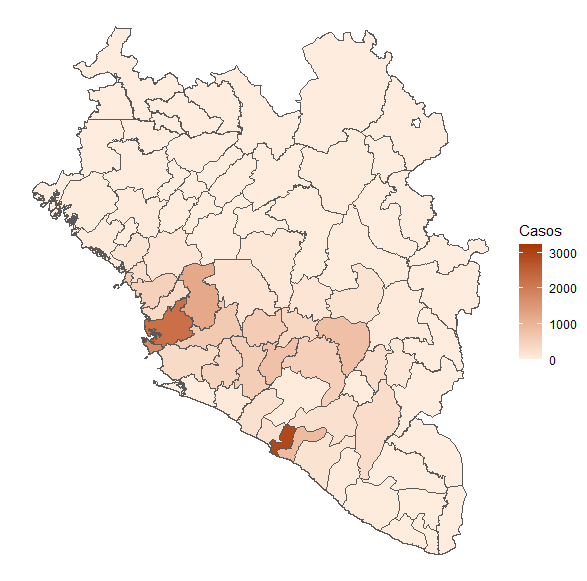
\includegraphics[width=0.9\textwidth]{images/raw_cases_ebola.png} % first figure itself
        \caption{Mapa dos casos brutos de ebola.}
    \end{minipage}\hfill
    \begin{minipage}{0.45\textwidth}
        \centering
        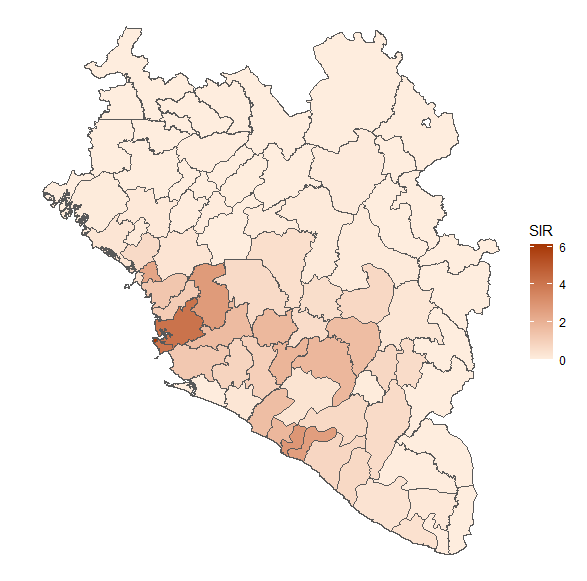
\includegraphics[width=0.9\textwidth]{images/SIR_ebola.png} % second figure itself
        \caption{Mapa da SIR para o caso do Ebola. A população suscetível foi considerada a população total.}
    \end{minipage}
\end{figure}

\begin{table}[h]
    \centering
    \begin{tabular}{|p{5cm} |p{5cm} |p{5cm} |}
    \hline
        Tipo de preditor & Abreviação & Descrição \\ \hline
        Demográfico & pdensMN & Densidade populacional (hab/km$^2$) \\\hline
       Demográfico &geconMN& Produção econômica média\\\hline
        Demográfico&geconMIN& Mínimo da produção econômica\\\hline
        Demográfico&geconMAX& Máximo da produção econômica\\\hline
        Demográfico&geconSTD& Desvio padrão da produção econômica\\\hline
        Demográfico&ttXkMN& Tempo de viagem média estimado para a cidade mais próxima com uma população de pelo menos $X \times 10.000$ habitantes, para $X = 50, 100$ e $500$\\\hline
        Climático&altMN& Altitude média\\\hline
        Climático&tempMN& Temperatura anual média\\\hline
        Climático&tempssMN&Sazonalidade média da temperatura\\\hline
        Climático&precMN& Precipitação anual média\\\hline
        Climático&precssMN&Sazonalidade média da precipitação \\\hline
        Filogenético&Introadmin& Número médio de introduções virais preditas usando fronteiras administrativas\\\hline
        Filogenético&Introdista& Número médio de introduções virais preditas usando fronteiras administrativas\\
        \hline
    \end{tabular}
    \caption{Preditores considerados para a modelagem da epidemia de Ebola. Todos os preditores contínuos foram padronizados subtraindo-se a média e dividindo pelo desvio-padrão.}
    \label{tab:ebola_predictors}
\end{table}


Para a modelar a contagem de casos utilizarei 6 modelos diferentes: Poisson Log-normal simples, Poisson Log-normal com ORLE e o modelo BYM2, e todos estes modelos novamente mas com a inclusão do esquema de seleção de variáveis SSVS de Kuo e Mallick. Para cada modelo também teremos o WAIC como comparativo, a eficiência em (ESS/s) e o erro médio quadrático à posteriori, disposta na \autoref{tab:posterior_summary_ebola}. Foi rodada uma única cadeia com 300.000 iterações, 200.000 de \textit{burnin} com parâmetro de thinning igual a 10 para cada modelo.

Os diagnósticos de cadeia não foram muito satisfatórios. A quantidade de amostras efetivas produzidas por rodada é bem baixa. Os parâmetros $\beta$ apresentaram alta autocorrelação, o que sinaliza convergência lenta. Apesar disso, os resultados em termos de WAIC e RMSE foram bons. Antes de comparara relevância das variáveis, um resultado interessante apresentado foi o BYM2 no cenário de seleção de variáveis. Aplicando o teste de Moran para cada covariável, apenas uma não apresenta forte estrutura espacial que foi a de densidade populacional. Todas as outras tiveram p-valor menor que 0.0001. O BYM2 acabou absorvendo toda a informação espacial, e nenhuma variável foi selecionada mais de 20 \% das vezes. No modelo com a inclusão de todas as variáveis o parâmetro $\rho$ se comportou de forma parecida com a priori uniforme, comportamento similar aos testes da \autoref{sec:spatial} de quando não havia resíduo espacial. Na seleção de variáveis, a média a posteriori de $\rho$ salta para 0.8, indicando forte associação espacial, e nenhuma variável foi selecionada. 

Por este motivo, utilizarei o modelo com ORLE para analisar a relevância de variáveis. Um ponto a se notar aqui é a alta correlação entre as covariáveis (\autoref{fig:corplot}), que afeta a interpretação dos resultados. outro problema está na convergência: a cadeia visita o espaço de modelos de forma bem lenta. A tendência observada foi de terem variáveis que sempre são selecionadas, e as outras variáveis sendo selecionadas esporadicamente. A cadeia consegue se desvencilhar do estado inicial. Para avaliar a situação melhor, rodei 400 cadeias em paralelo, observando as frequências de modelo escolhidas em cada uma. As cadeias começam todas de pontos diferentes: 100 delas começando de $\gamma = (0,\dots, 0)$, 100 delas começando em $\gamma = (1, \dots, 1)$, e o resto de algum ponto aleatório uniformemente escolhido em $\{0,1\}^p$. Apresento como resultado as médias à posteriori da indicadora de cada covariável:

\begin{table}[]
    \centering
    \begin{tabular}{|c|c|}
    \hline
            \textbf{Covariável}& \textbf{Média} \\ \hline
            geconMN  & 0.09  \\ \hline
            geconMIN  & 0.36  \\ \hline
            geconMAX  & 0.14  \\ \hline
            geconSTD  & 0.04  \\ \hline
            pdensMN  & 0.07  \\ \hline
            tt50kMN  & 0.20  \\ \hline
            tt100kMN  & 0.38  \\ \hline
            tt500kMN  & 0.18  \\ \hline
            altMN  & 0.21  \\ \hline
            tempMN & 0.33  \\ \hline
            tmpssMN & 0.42 \\ \hline
            precMN & 0.16 \\ \hline
            precssMN & 0.56  \\ \hline
            Introadmin & 0.04  \\ \hline
            Introdista & 0.03 \\ \hline
    \end{tabular}
    \caption{Médias \textit{à posteriori} das indicadoras das covariáveis para as múltiplas cadeias do modelo com ORLE.}
    \label{tab:posterior_gamma}
\end{table}



As análises do fator de Bayes não serão interessantes nesse cenário de fraca convergência da cadeia. Mas podemos gerar mapas da probabilidade \textit{à posteriori} da SIR ser maior do que 1, assim como realizar a predição das regiões sem casos. Aqui o modelo BYM2 mostra sua vantagem em relação ao BYM. A posteriori para $\tau_b$ é compatível com ambos os grafos de adjacências. Os resultados estão dispostos na \autoref{fig:pred}

\begin{figure}
    \centering
    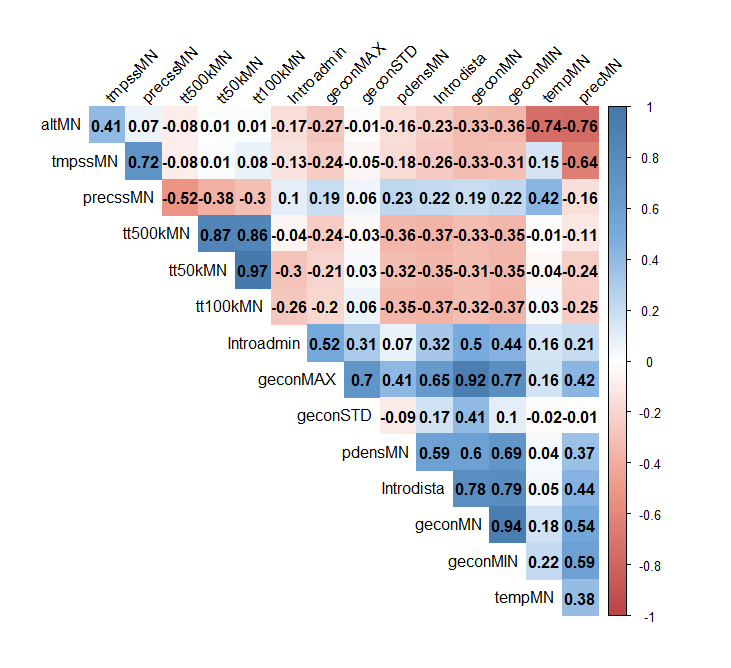
\includegraphics[width = 0.5\linewidth]{images/correlation_btwn_cov_ebola.png}
    \caption{Correlação entre as variáveis disponíveis para o estudo do Ebola. Destas, apenas a densidade populacional (pdensMN) não apresenta forte estrutura espacial.}
    \label{fig:corplot}
\end{figure}


\begin{table}
\centering
\begin{tabular}{@{}lrrcrrcccc@{}}\toprule
& SSVS & \phantom{ab}&  WAIC & \phantom{ab}& Eficiência & \phantom{ab}& Eficiência mínima & \phantom{ab}& RMSE\\

%\cmidrule{2-3} \cmidrule{5-6}
%& $Média$ & $(upp,lwr)$ && $Média$ & $(upp,lwr)$\\
\midrule
\textbf{Simples} & Não &&  5856.5 && 126.2 &&  30.4 && 139.9\\ 
\textbf{ORLE} & Não &&  459.7 && 145.1  &&  0.03 && 0.68\\ 
\textbf{BYM2} & Não &&  699.4 && 30.25  && 0.03 && 0.77\\
\textbf{Simples} & Sim &&  5670.6 && 6.26 && 0.165 && 141.0\\  
\textbf{ORLE} & Sim &&  475.5  &&  37.0 && 0.01  && 0.72\\ 
% var.s  0.6504600  0.6433667 0.1170732  0.4446273  0.90150079
\textbf{BYM2} & Sim &&  711.9 && 39.05 && 0.01 && 1.24\\

\bottomrule
\end{tabular}
    \caption{Comparativo dos 6 modelos usados para modelagem dos casos de Ebola. Eficiência (ESS por segundo) representa a eficiência média de todos os parâmetros da cadeia. Eficiência mínima é a menor eficiência encontrada. RMSE é a raiz do Erro Médio Quadrático.}
    \label{tab:posterior_summary_ebola}
\end{table}


\begin{figure} % "[t!]" placement specifier just for this example
\begin{subfigure}{0.38\textwidth}
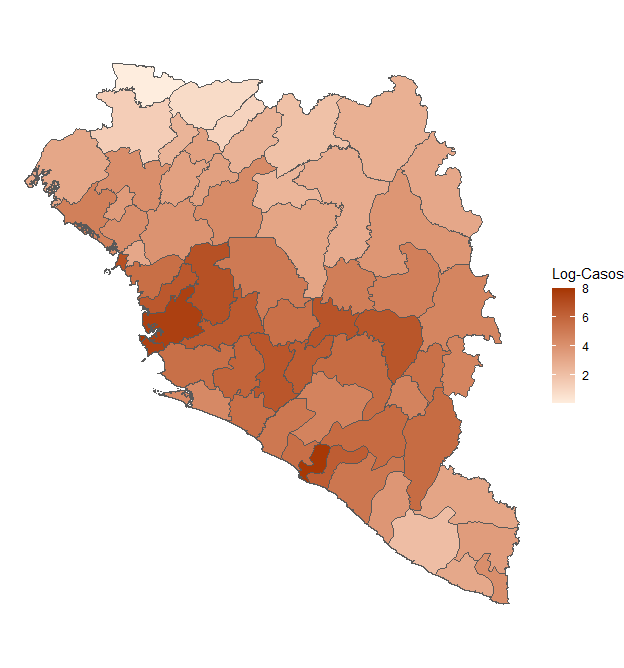
\includegraphics[width=\linewidth]{images/posterior_mean_simples.png}
\caption{Modelo simples} \label{fig:a}
\end{subfigure}\hspace*{\fill}
\begin{subfigure}{0.38\textwidth}
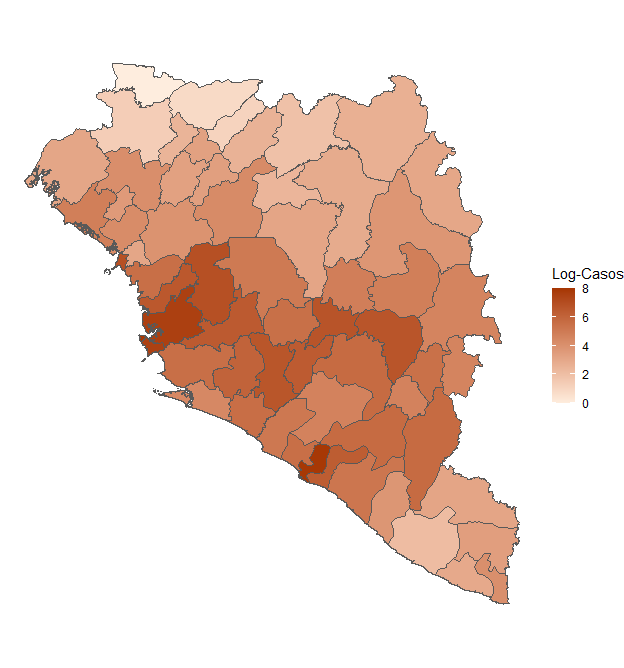
\includegraphics[width=\linewidth]{images/posterior_mean_ssvs.png}
\caption{Modelo simples com seleção de variáveis} \label{fig:b}
\end{subfigure}

\medskip
\begin{subfigure}{0.38\textwidth}
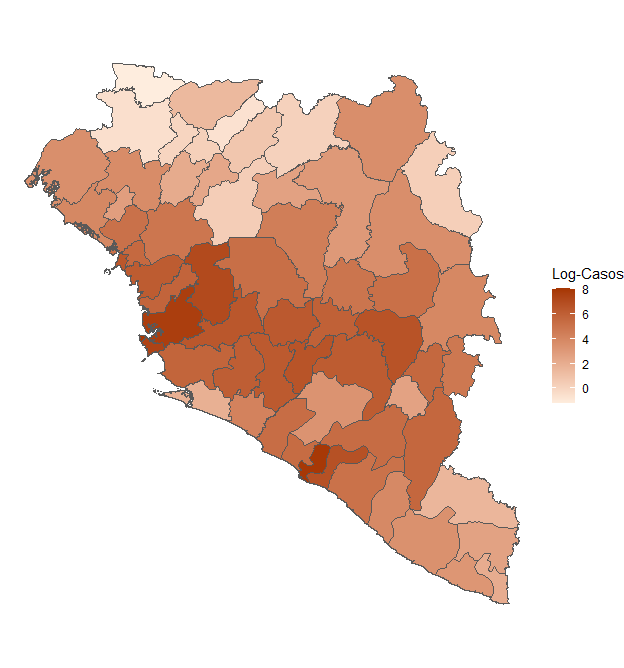
\includegraphics[width=\linewidth]{images/posterior_mean_orle.png}
\caption{Modelo com ORLE} \label{fig:c}
\end{subfigure}\hspace*{\fill}
\begin{subfigure}{0.38\textwidth}
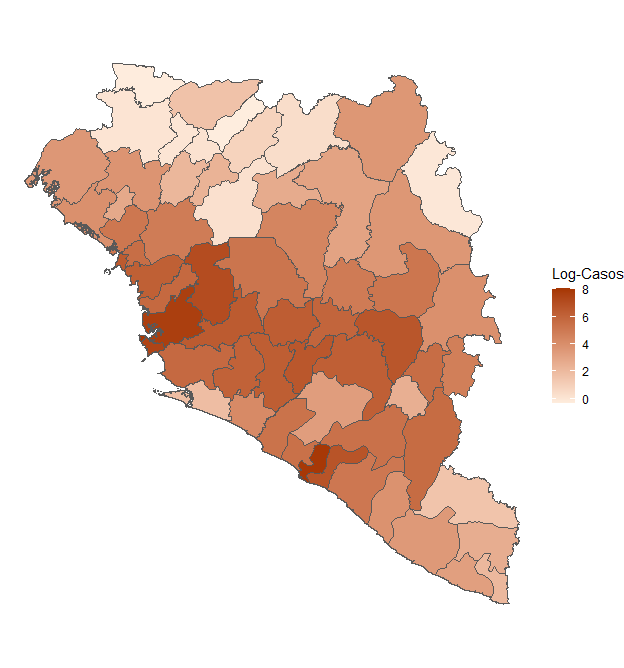
\includegraphics[width=\linewidth]{images/posterior_mean_orle_ssvs.png}
\caption{Modelo com ORLE e seleção de variáveis} \label{fig:d}
\end{subfigure}

\medskip
\begin{subfigure}{0.38\textwidth}
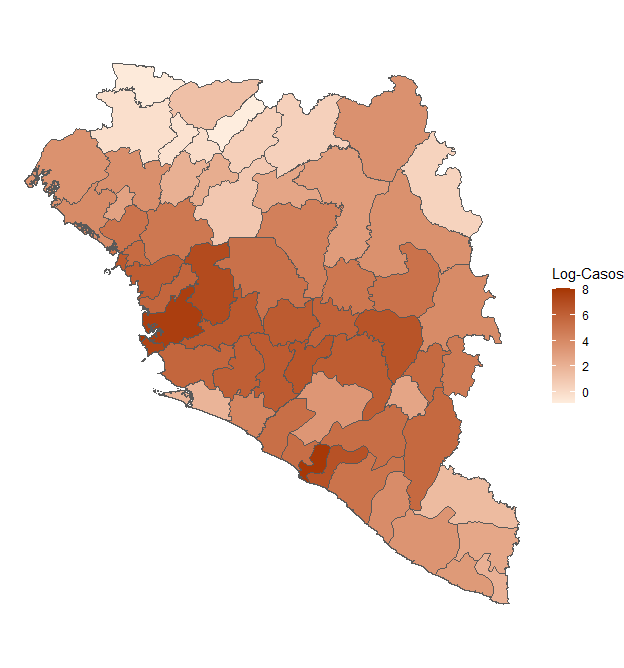
\includegraphics[width=\linewidth]{images/posterior_mean_bym2.png}
\caption{Modelo BYM2} \label{fig:e}
\end{subfigure}\hspace*{\fill}
\begin{subfigure}{0.38\textwidth}
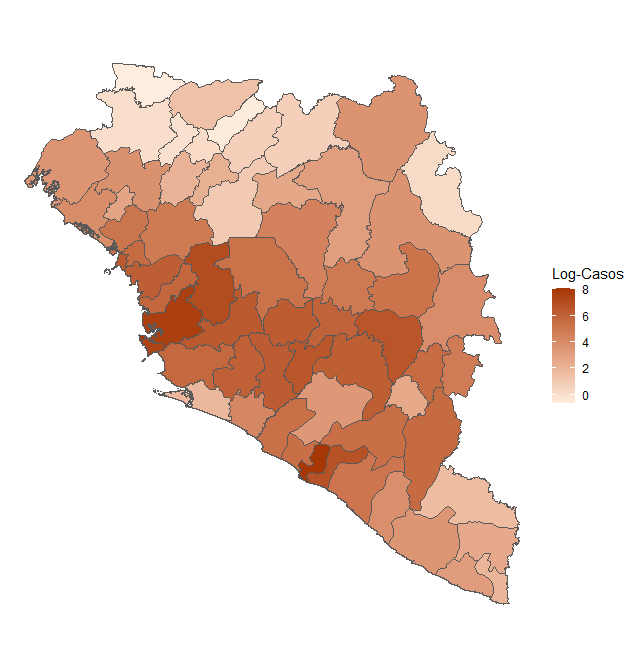
\includegraphics[width=\linewidth]{images/posterior_mean_bym2_ssvs.png}
\caption{Modelo BYM2 com seleção de variáveis} \label{fig:f}
\end{subfigure}

\caption{Mapa do log da média a posteriori de casos para os seis modelos de contagem de casos utilizados} \label{fig:ebola_posterior_maps}
\end{figure}

\begin{figure}
    \centering
    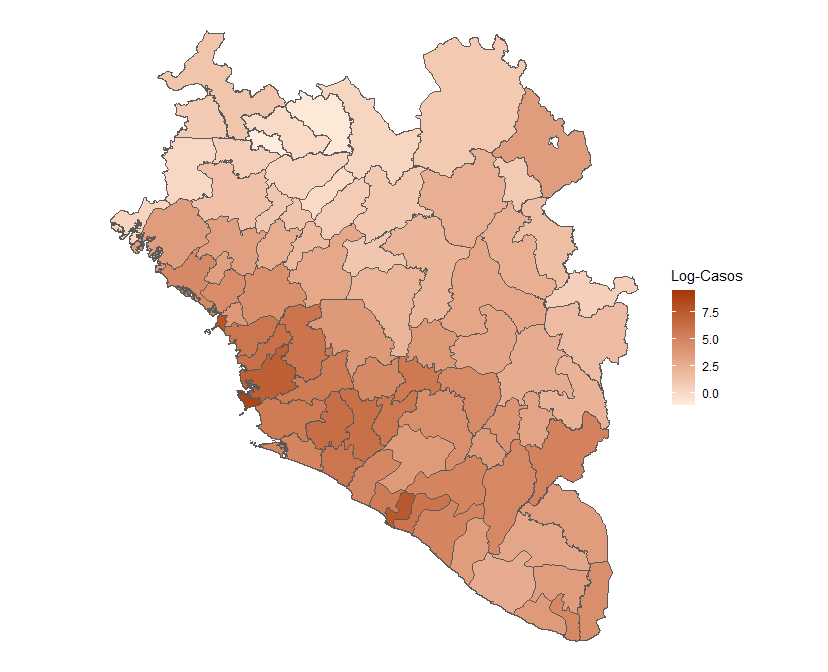
\includegraphics[width = 0.8\linewidth]{images/posterior_predicitve_bym2.png}
    \caption{Preditiva à posteriori, incluindo regiões agora que não tiveram casos registrados.}
    \label{fig:pred}
\end{figure}



\chapter{Conclusão}

Modelos hierárquicos Bayesianos são um forte aliado de qualquer pesquisador da área de epidemiologia. Uma de suas grandes vantagens é ser altamente interpretável, e poder acomodar todo tipo de hipótese dentro de sua formulação. Em especial, para epidemiologia espacial conseguimos acoplar a necessidade por dependência espacial, que está presente em todas as coisas, como diz a Primeira Lei da Geografia de \cite{Tobler1970}. Conseguimos acoplar também uma análise de regressão, uma poderosa ferramente estatística, mas que deve ser tratada com cautela. Neste trabalho tivemos complicações com o modelo do Ebola, não obtendo a desejada convergência da cadeia. Apesar do modelo ter tido bons resultados em termos de RMSE, resultados estatísticos não podem ser traçados. 

Possíveis correções e sugestões para futuros trabalhos são: analisar diferentes amostradores e sua eficiência comparada aos amostrados base do NIMBLE. O próprio NIMBLE já possui em versão beta amostradores por HMC (Hamiltonian Monte Carlo). Outra opção é o INLA (INtegrated Nested Laplace Approximation ). Mesmo que tivessemos conseguido um bom amostrador, temos o problema da alta correlação entre as covariáveis do ebola, que pode distribuir a importância dessas variáveis e levar à interpretação errada de parâmetros. Algumas sugestões são adicionar ao modelo através das prioris, estruturas que permitam a agregação de variáveis correlacionadas, como em \cite{IsingDP}. Uma terceira indagação para o futuro é sobre quais seriam os melhores diagnósticos de cadeia para este cenário. Veja que no conjunto de dados do Ebola, apesar de não termos atingido convergência da cadeia, obtivemos bons resultados de RMSE, o que poderia levar a conclusões erradas sobre a eficácia do modelo. 

% -----------------------------------
% ELEMENTOS PÓS-TEXTUAIS
% -----------------------------------
\postextual
% ----------------------------------

%\bibliography{biblio}
\printbibliography

%\glossary

% ----------------------------------------------------------
% Apêndices
% ----------------------------------------------------------

% ---
% Inicia os apêndices
% ---
 \begin{apendicesenv}

% % Imprime uma página indicando o início dos apêndices
\partapendices
\chapter{Gaussian Markov Random Fields}\label{ap: IGMRF}

\textit{Gaussian Markov Random Fields} (GMRF's) são objetos simples: vetores aleatórios (de dimensão finita) seguindo uma distribuição normal multivariada. Apesar disso, nosso interesse está em versões mais restritas das GMRF's, que satisfazem certas condições de independência (daí o cunho \textit{Markov}).

\begin{definition}
\label{def:GMRF}
Seja $\x = (x_1, \dots, x_n)^T$ um vetor aleatório com distribuição normal de média $\mathbf{\mu}$ e matriz de covariância $\mathbf{\Sigma}$. Defina o grafo $G = (V,E)$, onde $V=\{1,\dots, n\}$, tal que não há aresta conectando dois nós $i$ e $j$ se, e somente se, $x_i \perp x_j|\x_{-ij}$. Dizemos que $\x$ é um GMRF com respeito ao grafo $G$.
\end{definition}

A matriz de precisão da normal multivariada explicita algumas características de independência condicional. Em especial, temos o teorema abaixo:

\begin{theorem}
\label{thm: nullQ}
Seja $\x$ um vetor com distribuição normal de média $\mathbf{\mu}$ e matriz de precisão $Q \succ 0$. Então, para $i \neq j$,
\begin{equation}
    x_i \perp x_j|\x_{-ij} \iff Q_{ij} = 0.
\end{equation}
\end{theorem}

\textit{Prova.} Para isso, particionamos o vetor $\x = (x_i, x_j, \x_{-ij})$ e utilizamos do critério da fatorização. Sem perda de generalidade, assuma $\mathbf{\mu} = 0$. A densidade conjunta de $\x$ pode ser expressa como:

\begin{flalign}
    \pi(\x) = \pi(x_i, x_j, \x_{-ij}) & \propto \exp (-\frac{1}{2}\x^T Q \x) \\ \nonumber
    & \propto \exp \left(-\frac{1}{2} \sum_{k,l} x_kQ_{k,l}x_l\right) \\ \nonumber
    & \propto \exp \left(\underbrace{-\frac{1}{2}x_ix_j(Q_{ij}+Q_{ji})}_{\text{Termo 1}} \underbrace{-\frac{1}{2} \sum_{\{k,l\} \neq \{i,j\}} x_kQ_{kl}x_l}_{\text{Termo 2}}\right).
\end{flalign}

Veja que o Termo 2 não envolve o produto $x_ix_j$, enquanto o Termo 1 envolve $x_ix_j$ se, e somente se, $Q_{ij} \neq 0$. Então, se vale que $Q_{ij} = 0$, é possível fatorar $\pi(\x)$ como:
\begin{equation}
    \pi(x_i, x_j, \x_{-ij}) = f(x_i,\x_{-ij})g(x_j,\x_{-ij}).
\end{equation}

Pelo critério de fatorização, $x_i$ e $x_j$ são independentes se, e somente se, $Q_{ij} = 0$ $\qed$

Faz sentido então caracterizar os GMRF's através de sua matriz de precisão. Considere então a seguinte reformulação de \ref{def:GMRF}:

\begin{definition}
Um vetor aleatório $\x = (x_1,\dots, x_n) \in \mathbb{R}^n$ é um GMRF com respeito ao grafo $G = (V,E)$ com média $\mathbf{\mu}$ e matriz de precisão $\mathbf{Q} \succ 0$ se, e somente se, sua densidade é da forma:

\begin{equation}
    \label{eq: GMRFdensity}
    \pi(\x) = (2\pi)^{-n/2}|\mathbf{Q}|^{1/2} \exp(-\frac{1}{2}\left(\x-\mu)^T\mathbf{Q}(\x-\mu)\right),
\end{equation}
e
\[Q_{ij} \neq 0 \iff \{i,j\} \in E \quad \forall i \neq j.\]

\end{definition}

Uma forma alternativa de caracterizar um GMRF é através das condicionais completas. Essa abordagem foi desenvolvida por Besag e os modelos são abreviados como CAR (\textit{conditional autoregressions}). Então suponha que para o vetor de dados $\textbf{x} = (x_1, \dots, x_n)$ especificamos as condicionais completas como normais de parâmetros:

\begin{flalign}
\label{def:fullconditionals}
        \ev(x_i|\x_{-i}) &= \mu_i - \sum_{j:j \sim i} \beta_{ij}(x_j - \mu_j),\\
            \var(x_i|\x_{-i}) &= \frac{1}{\kappa_i} > 0.
\end{flalign}

Aqui, $\sim$ [e uma relação de simetria definida implicitamente pelos termos não-nulos de $\boldsymbol{\beta}$. Essas condicionais completas devem ser consistentes de modo a gerar a densidade conjunta $\pi(\x)$. De fato, veja que se escolhermos as entradas da matriz de precisão como:
\[Q_{ii} = \kappa_i \quad \text{and} \quad Q_{ij} = \kappa_i\beta_{ij}\]
com a condição de Q simétrica, ou seja,
\[\kappa_i\beta_{ij} = \kappa_j\beta_{ji}\]
temos um candidato a densidade conjunta. Este candidato a densidade é único, e para mostrar isso precisamos do seguinte lema.

\begin{lemma}[Lema de Brook]
\label{lema:brook}

Seja $\pi(\x)$ a densidade de $\x \in \R^n$ e defina o suporte dessa densidade como o conjunto $\Omega = \{\x \in \R^n: \pi(\x) > 0\}$. Se $\x,\x' \in \Omega$, então:

\begin{flalign}
\label{eq:brook}
        \frac{\pi(\x)}{\pi(\x')} &= \prod_{i=1}^n \frac{\pi(x_i|x_1,\dots,x_{i-1},x'_{i+1}, \dots,x'_{n})}{\pi(x'_i|x_1,\dots,x_{i-1},x'_{i+1}, \dots,x'_{n})} \\
\label{eq:brook2}
         &= \prod_{i=1}^n \frac{\pi(x_i|x'_1,\dots,x'_{i-1},x_{i+1}, \dots,x_{n})}{\pi(x'_i|x'_1,\dots,x'_{i-1},x_{i+1}, \dots,x_{n}}
\end{flalign}
\end{lemma}

\textit{Demostração.} Como estamos dentro do suporte da distribuição, podemos usar as definições de densidade condicional para obter a seguinte relação:

\[\frac{\pi(x_n|x_1,\dots,x_{n-1})\pi(x_1,\dots,x_{n-1})}{\pi(x'_n|x_1,\dots,x_{n-1})\pi(x_1,\dots,x_{n-1})} = \frac{\pi(x_1,\dots,x_{n})}{\pi(x_1,\dots,x'_{n})}\]

que nos permite expressar a densidade conjunta como:
\[\pi(x_1,\dots,x_{n}) = \frac{\pi(x_n|x_1,\dots,x_{n-1})}{\pi(x'_n|x_1,\dots,x_{n-1})} \cdot
\pi(x_1,\dots,x_{n-1}, x'_n).\]
Podemos da mesma forma expressar o último termo da equação acima como 
\[\pi(x_1,\dots,x_{n-1}, x'_n) = \frac{\pi(x_{n-1}|x_1,\dots,x_{n-2},x'_n)}{\pi(x'_{n-1}|x_1,\dots,x_{n-2},x'_n)} \cdot
\pi(x_1,\dots,x_{n-2},x'_{n-1}, x'_n).\]
Substituindo na densidade conjunta
\[\pi(x_1,\dots,x_{n}) = \frac{\pi(x_n|x_1,\dots,x_{n-1})}{\pi(x'_n|x_1,\dots,x_{n-1})} \cdot \frac{\pi(x_{n-1}|x_1,\dots,x_{n-2},x'_n)}{\pi(x'_{n-1}|x_1,\dots,x_{n-2},x'_n)} \cdot
\pi(x_1,\dots,x_{n-2},x'_{n-1}, x'_n).\]
Basta então repetir o procedimento até o termo à direita se tornar a densidade conjunta de $\x' \qed$.

Com isso, se fixarmos $\x'$, obtemos a densidade de $\x$ a menos de uma constante de proporcionalidade. 

\begin{theorem}
Dadas as n condicionais completas como em \ref{def:fullconditionals}, então $\x$ é um GMRF com média $\mu$ e matriz de precisão $Q = (Q_{ij})$, onde
\[Q_{ij} = \left\{\begin{split}
\kappa_i\beta_{ij} \quad i \neq j \\
 \kappa_i \quad i = j\\ 
\end{split}\right.\]
com $\kappa_i\beta_{ij} = \kappa_j\beta_{ij}$ e $Q \succ 0$.

\end{theorem}

\textit{Demonstração.} Sem perda de generalidade, assuma $\mu = 0$ e  fixe $\x' = 0$ no Lema de Brook. Então o log de \ref{eq:brook} pode ser simplificado para:
\begin{equation}
    \log \frac{\pi(\x)}{\pi(0)} = -\frac{1}{2}\sum_{i=1}^{n}\kappa_ix_i^2 -\sum_{i=2}^n \sum_{j=1}^{i-1}\kappa_i\beta_{ij}x_ix_j,
\end{equation}

e \ref{eq:brook2} para
\begin{equation}
    \log \frac{\pi(\x)}{\pi(0)} = -\frac{1}{2}\sum_{i=1}^{n}\kappa_ix_i^2 -\sum_{i=1}^{n-1} \sum_{j=i+1}^{n}\kappa_i\beta_{ij}x_ix_j.
\end{equation}
Para isso, basta ver como cada termo do produtório se comporta

\[\prod_{i=1}^n \frac{\pi(x_i|x'_1,\dots,x'_{i-1},x_{i+1}, \dots,x_{n})}{\pi(x'_i|x'_1,\dots,x'_{i-1},x_{i+1}, \dots,x_{n})} = \exp\left( -\frac{\kappa_i}{2}(x_i^2 -2x_i[\sum_{\substack{j:i\sim j \\ j < i}}\beta_{ij}x'_j + \sum_{\substack{j:i\sim j \\ j > i}}\beta_{ij}x_j])  \right).\]

\[\prod_{i=1}^n \frac{\pi(x_i|x_1,\dots,x_{i-1},x'_{i+1}, \dots,x'_{n})}{\pi(x'_i|x_1,\dots,x_{i-1},x'_{i+1}, \dots,x'_{n})} = \exp\left( -\frac{\kappa_i}{2}(x_i^2 -2x_i[\sum_{\substack{j:i\sim j \\ j > i}}\beta_{ij}x'_j + \sum_{\substack{j:i\sim j \\ j < i}}\beta_{ij}x_j])  \right).\]

Como ambas devem ser iguais, segue que $\kappa_i\beta_{ij} = \kappa_j\beta_{ij}$, para $i \neq j$. A densidade de $\x$ então pode ser expressa como
\[\log \pi(\x) = \text{const} - \frac{1}{2}\sum_{i = 1}^n \kappa_ix_i^2 - \frac{1}{2}\sum_{i \neq j}\kappa_i\beta_{ij}x_ix_j. \quad \qed\]





\chapter{Intrinsic Gaussian Markov Random Fields}

Neste apêndice introduzo um tipo especial de GMRF chamadas de IGMRF, Campos Gaussianos Aleatórios de Markov Intrínsecos. Antes de começar a falar sobre IGMRF's, precisamos enunciar algumas definições de álgebra linear.

Primeiramente, o \textit{núcleo} ou espaço nulo de uma matriz $\mathbf{A}$ é o conjunto de todos os vetores $\mathbf{x}$ tais que $\mathbf{Ax = 0}$. A \textit{nulidade} é a dimensão do núcleo. Para uma matriz $n \times m$ o \textit{posto} é definido como $\min (m,n) = k$, onde $k$ é a nulidade de $\mathbf{A}$. Para uma matriz singular, i.e, não inversível, com nulidade $k$, denotamos $|\mathbf{A}|^*$ o produto dos $n-k$ autovalores não nulos de $\mathbf{A}$. 

Com isso, podemos definir o que é uma IGMRF de primeira ordem.

\begin{definition}
Seja $\mathbf{Q}$ uma matriz $n \times n$ semi-positiva definida com posto $n - k > 0$. Então $\mathbf{x} = (x_1, \dots, x_n)^T$ é uma GMRF imprópria de posto $n-k$ com parâmetros $(\mathbf{\mu}, \mathbf{Q})$, se sua densidade é
\begin{equation}
    \pi(\mathbf{x}) = (2\pi)^{\frac{-(n-k)}{2}}(|\mathbf{Q}|^* )^{1/2} \exp \left(  -\frac{1}{2} \mathbf{(x-\mu)^TQ^T(x-\mu)} \right).
\end{equation}
\end{definition}


Uma GMRF intrinseca é uma GMRF imprópria de rank $n-1$, onde o vetor $\mathbf{1} = (1, \dots, 1)$ gera o espaço nulo de $\mathbf{Q}$. Ou seja, $\mathbf{Q1} = 0$. Já é possível ver que a densidade de uma IGMRF é invariante a adição de uma constante $c\mathbf{1 = c}$, basta olhar o núcleo da exponencial na densidade.



\begin{equation*}
\begin{split}
        \mathbf{(x-\mu +c)^TQ^T(x-\mu+c)} &= \mathbf{(x-\mu)^TQ^T(x-\mu) + c^TQ^T(x-\mu)} \\
                                         &+   \mathbf{(x-\mu)^TQ^Tc + c^TQ^Tc} \\
                                        &= \mathbf{(x-\mu)Q^T(x-\mu)} 
\end{split}
\end{equation*}

É importante notar isso para impor restrições para a IGMRF somar zero. Caso contrário, pode haver confusão com o intercepto.

\end{apendicesenv}
% ---

% ----------------------------------------------------------
% Anexos
% ----------------------------------------------------------

% \begin{anexosenv}

% \partanexos

% \end{anexosenv}
"
%---------------------------------------------------------------------
% ÍNDICE REMISSIVO
%---------------------------------------------------------------------
\phantompart
\printindex

\end{document}